\documentclass[12pt,a4paper]{report}

% -----------------------------------------------------------------------------
% CẤU HÌNH GÓI VÀ BỐ CỤC TRANG
% -----------------------------------------------------------------------------
\usepackage[utf8]{inputenc}
\usepackage[T5,T1]{fontenc}
\usepackage[vietnamese,english]{babel}
\usepackage[a4paper, top=2.5cm, bottom=2.5cm, left=3cm, right=2cm]{geometry}

\usepackage{amsmath,amssymb,amsfonts,amsthm}
\usepackage{booktabs}
\usepackage{graphicx}
\usepackage{subcaption}
\usepackage{multirow}
\usepackage{array}
\usepackage{tabularx}
\usepackage{xcolor}
\usepackage{url}
\usepackage{setspace}
\usepackage{longtable}
\usepackage{algorithm}
\usepackage{algpseudocode}
\usepackage{tikz}
\usetikzlibrary{calc}

% Cấu hình liên kết hyperref
\usepackage[
    colorlinks=true,
    linkcolor=black,
    citecolor=blue,
    urlcolor=blue,
    bookmarks=true,
    bookmarksnumbered=true,
    plainpages=false,
    pdfpagelabels=true
]{hyperref}

% Định nghĩa môi trường định lý
\newtheorem{theorem}{Định lý}[chapter]
\newtheorem{lemma}[theorem]{Bổ đề}
\newtheorem{definition}{Định nghĩa}[chapter]
\newtheorem{proposition}[theorem]{Mệnh đề}

% Đánh số mục theo chuẩn format: Chapter.Section. (ví dụ: 1.1., 1.2.)
\renewcommand{\thesection}{\thechapter.\arabic{section}.}
\renewcommand{\thesubsection}{\thechapter.\arabic{section}.\arabic{subsection}.}

% Định dạng hiển thị thuật toán
\renewcommand{\listalgorithmname}{Danh mục Thuật toán}
\floatname{algorithm}{Thuật toán}

% Giãn dòng chuẩn học thuật
\onehalfspacing

\begin{document}
\selectlanguage{vietnamese}

% -----------------------------------------------------------------------------
% TRANG BÌA (TITLE PAGE) THEO FORMAT CHUẨN BÁO CÁO UET
% -----------------------------------------------------------------------------
\hypersetup{pageanchor=false}
\begin{titlepage}
% Khung viền bao quanh trang bìa chuẩn mẫu UET
\begin{tikzpicture}[remember picture, overlay]
    \draw[line width = 2pt] 
        ($(current page.north west) + (2.0cm, -1.5cm)$) 
        rectangle 
        ($(current page.south east) + (-1.5cm, 1.5cm)$);
\end{tikzpicture}
\begin{center}
    {\large \textbf{ĐẠI HỌC QUỐC GIA HÀ NỘI}}\\[0.2cm]
    {\large \textbf{TRƯỜNG ĐẠI HỌC CÔNG NGHỆ}}\\[1.0cm]
    
    
\includegraphics[width=3.6cm]{figures/uet_logo.png}\\[1.2cm]
    
    {\Large \textbf{BÁO CÁO BÀI TẬP LỚN MÔN HỌC}}\\[0.4cm]
    {\large \textbf{HỌC PHẦN: CÁC VẤN ĐỀ HIỆN ĐẠI TRONG KHOA HỌC MÁY TÍNH}}\\[1.2cm]
    
    \rule{\textwidth}{1.2pt}\\[0.5cm]
    {\LARGE \bfseries NGHIÊN CỨU THỰC NGHIỆM CÁC KỸ THUẬT MÃ HÓA SAT VÀ SO SÁNH ĐA MÔ HÌNH (SAT, CP, MIP) CHO BÀI TOÁN N-QUEENS}\\[0.3cm]
    \rule{\textwidth}{1.2pt}\\[2.0cm]
    
    \begin{tabular}{ll}
        \textbf{Giảng viên hướng dẫn:} & TS. Tô Văn Khánh \\
        \textbf{Học phần:}             & INT3011E 3 \\
        \textbf{Sinh viên thực hiện:}   & Trần Nhật Hưng -- 24021507 \\
    \end{tabular}
    
    \vfill
    {\large \textbf{HÀ NỘI, 2026}}
\end{center}
\end{titlepage}

% -----------------------------------------------------------------------------
% PHẦN ĐẦU (FRONT MATTER)
% -----------------------------------------------------------------------------
\hypersetup{pageanchor=true}
\pagenumbering{roman}
\setcounter{page}{1}

% Mục lục
\tableofcontents
\cleardoublepage

% Danh mục bảng
\listoftables
\cleardoublepage

% Danh mục hình vẽ
\listoffigures
\cleardoublepage

% Danh mục thuật toán
\listofalgorithms
\cleardoublepage

% Danh mục từ viết tắt
\chapter*{Danh mục Từ viết tắt}
\addcontentsline{toc}{chapter}{Danh mục Từ viết tắt}

\begin{table}[h]
\centering
\begin{tabular}{p{3.2cm} p{11.8cm}}
\toprule
\textbf{Từ viết tắt} & \textbf{Ý nghĩa / Tên đầy đủ} \\
\midrule
\textbf{ALO} & At-Least-One (Ràng buộc Có ít nhất một) \\
\textbf{AMO} & At-Most-One (Ràng buộc Có nhiều nhất một) \\
\textbf{CDCL} & Conflict-Driven Clause Learning (Thuật toán học mệnh đề theo xung đột) \\
\textbf{CNF} & Conjunctive Normal Form (Dạng chuẩn hội) \\
\textbf{CP} & Constraint Programming (Lập trình ràng buộc) \\
\textbf{CSP} & Constraint Satisfaction Problem (Bài toán thỏa mãn ràng buộc) \\
\textbf{DPLL} & Davis-Putnam-Logemann-Loveland (Thuật toán tìm kiếm SAT kinh điển) \\
\textbf{GAC} & Generalized Arc Consistency (Tính nhất quán cung tổng quát) \\
\textbf{ILP} & Integer Linear Programming (Quy hoạch tuyến tính nguyên) \\
\textbf{LBD} & Literal Block Distance (Khoảng cách khối biến logic) \\
\textbf{MIP} & Mixed Integer Programming (Quy hoạch tuyến tính nguyên hỗn hợp) \\
\textbf{OOM} & Out-Of-Memory (Tràn bộ nhớ vật lý) \\
\textbf{SAT} & Boolean Satisfiability Problem (Bài toán thỏa mãn logic mệnh đề) \\
\textbf{UNSAT} & Unsatisfiable (Không thỏa mãn) \\
\textbf{UP} & Unit Propagation (Lan truyền đơn vị) \\
\textbf{VSIDS} & Variable State Independent Decaying Sum (Heuristic phân nhánh biến) \\
\textbf{2WL} & Two-Watched Literals (Kỹ thuật theo dõi hai biến đại diện) \\
\bottomrule
\end{tabular}
\end{table}
\cleardoublepage

% Lời mở đầu
\chapter*{Lời mở đầu}
\addcontentsline{toc}{chapter}{Lời mở đầu}

Trong bối cảnh khoa học máy tính và trí tuệ nhân tạo phát triển vượt bậc, các \textit{Phương pháp Hình thức} (Formal Methods) và các mô hình tính toán khai báo chính xác đóng vai trò then chốt trong việc kiểm thử, xác minh hệ thống phần cứng, phần mềm, cũng như giải quyết các bài toán tối ưu hóa tổ hợp quy mô lớn \cite{clarke1996formal}. Trong đó, hai trường phái tính toán nổi bật nhất bao gồm:

\begin{itemize}
    \item \textbf{Lập trình Ràng buộc (Constraint Programming - CP):} Mô hình hóa bài toán dựa trên các ràng buộc logic hoặc toán học giữa các biến nguyên và sử dụng thuật toán lan truyền miền giá trị toàn cục để cắt tỉa không gian tìm kiếm \cite{barber2003introduction}.
    \item \textbf{Thỏa mãn Logic Mệnh đề (Boolean Satisfiability - SAT):} Xác định xem một công thức logic Boolean có thể được thỏa mãn hay không. Mặc dù SAT là bài toán NP-đầy đủ đầu tiên được chứng minh trong lý thuyết độ phức tạp \cite{cook1971complexity}, sự trỗi dậy của các bộ giải SAT CDCL hiện đại đã biến SAT thành một công cụ vạn năng giải quyết bài toán thực tế chứa hàng triệu biến trong thời gian mili-giây \cite{marques2008practical,biere2009handbook}.
\end{itemize}

Bài toán \textbf{$N$-Queens (Xếp $N$ quân hậu)} là bài toán chuẩn mực (benchmark) kinh điển được sử dụng phổ biến nhất để kiểm chuẩn và đánh giá năng lực của các thuật toán tìm kiếm và giải quyết ràng buộc tổ hợp \cite{letavec2002nqueens,rivin1994nqueens}. Việc mở rộng bài toán lên kích thước lớn ($N \ge 500$, tương ứng bàn cờ chứa hàng triệu ô cờ) đặt ra thách thức bùng nổ tổ hợp cực độ đối với các bộ giải.

Trong báo cáo này, chúng tôi tập trung nghiên cứu chuyên sâu về các kỹ thuật mã hóa ràng buộc At-Most-One (AMO) tối ưu trong SAT Solving (gồm Binomial, Sequential Counter, Binary, Commander Variable, và 2-Product), đồng thời mở rộng thiết lập thực nghiệm đối đầu đa mô hình (Cross-Paradigm Benchmark) giữa ba trường phái giải chính xác: SAT Solving (PySAT Glucose4), Lập trình Ràng buộc CP (Google OR-Tools, IBM ILOG CPLEX CP Optimizer), và Quy hoạch Tuyến tính Nguyên MIP (Gurobi Optimizer, IBM ILOG CPLEX MIP) trên chuỗi 15 mốc kích thước từ $N = 4$ đến $N = 1000$.

Báo cáo được tổ chức thành 5 chương chính như sau:
\begin{itemize}
    \item \textbf{Chương 1: Giới thiệu} -- Định nghĩa bài toán N-Queens, các quy tắc, ứng dụng thực tế và phân tích các thuật toán giải truyền thống (Quay lui, Nhánh cận) cùng hướng tiếp cận SAT.
    \item \textbf{Chương 2: Cơ sở lý thuyết} -- Giới thiệu logic mệnh đề, dạng chuẩn hội (CNF), kiến trúc bộ giải SAT CDCL hiện đại, và nguyên lý của 4 kỹ thuật mã hóa AMO tối ưu.
    \item \textbf{Chương 3: Phương pháp đề xuất và Mô hình hóa} -- Chi tiết hóa các công thức toán học mã hóa bài toán N-Queens trong SAT, CP và MIP.
    \item \textbf{Chương 4: Thực nghiệm và Đánh giá kết quả} -- Trình bày kết quả đo đạc 15 mốc kích thước, các bảng số liệu, biểu đồ so sánh và phân tích sâu sắc các hiện tượng thực nghiệm (sự bùng nổ mệnh đề Binomial, nghịch lý Sequential Counter, ưu thế của CPLEX CP và MIP).
    \item \textbf{Chương 5: Kết luận} -- Tổng kết toàn diện các kết quả nghiên cứu và đúc kết khuyến nghị lựa chọn kỹ thuật mã hóa, bộ giải tối ưu.
\end{itemize}

\cleardoublepage

% -----------------------------------------------------------------------------
% PHẦN THÂN BÁO CÁO (MAIN BODY)
% -----------------------------------------------------------------------------
\pagenumbering{arabic}
\setcounter{page}{1}

% =============================================================================
% CHƯƠNG 1: GIỚI THIỆU
% =============================================================================
\chapter{Giới thiệu}
\label{chap:intro}

\section{Định nghĩa bài toán}
\label{sec:problem_def}
Bài toán $N$-Queens (Xếp $N$ quân hậu) là bài toán kinh điển trong lĩnh vực trí tuệ nhân tạo, tối ưu hóa tổ hợp và suy luận tự động \cite{letavec2002nqueens}. Được kỳ thủ Max Bezzel đề xuất lần đầu tiên vào năm 1848 cho bàn cờ $8 \times 8$ \cite{bezzel1848} và được Franz Nauck tổng quát hóa cho kích thước $N \times N$ vào năm 1850 \cite{nauck1850}, mục tiêu của bài toán là tìm cách đặt $N$ quân hậu trên bàn cờ kích thước $N \times N$ sao cho không có bất kỳ hai quân hậu nào có thể tấn công lẫn nhau.

\begin{figure}[htbp]
    \centering
    \begin{subfigure}[b]{0.45\textwidth}
        \centering
        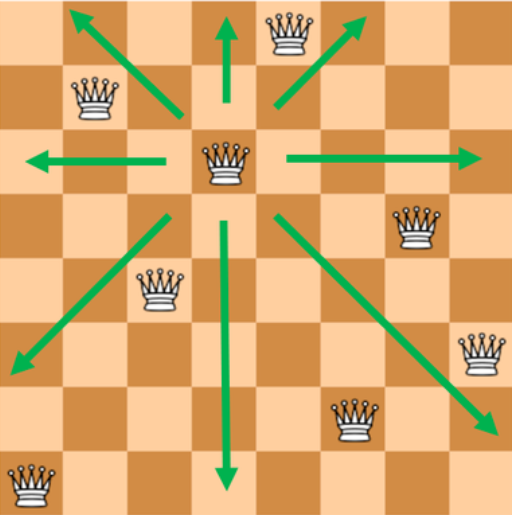
\includegraphics[width=0.88\linewidth]{figures/nqueens_valid.png}
        \caption{Cấu hình nghiệm hợp lệ}
        \label{fig:valid_queen}
    \end{subfigure}
    \hfill
    \begin{subfigure}[b]{0.45\textwidth}
        \centering
        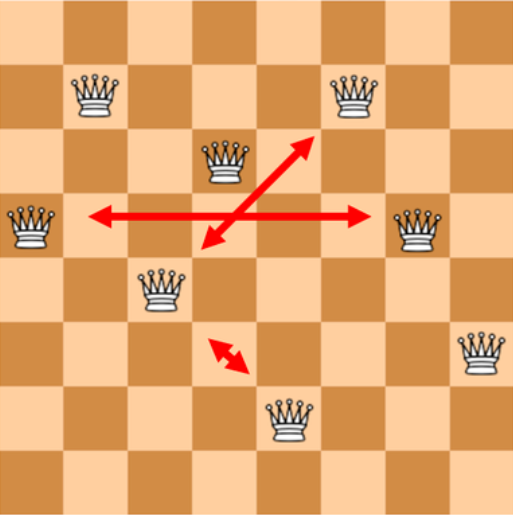
\includegraphics[width=0.88\linewidth]{figures/nqueens_invalid.png}
        \caption{Cấu hình vi phạm ràng buộc}
        \label{fig:invalid_queen}
    \end{subfigure}
    \caption{Minh họa cấu hình nghiệm hợp lệ và cấu hình vi phạm trên bàn cờ $N$-Queens.}
    \label{fig:nqueens_illustration}
\end{figure}

Hình~\ref{fig:nqueens_illustration} thể hiện sự khác biệt trực quan giữa một cấu hình hợp lệ và một cấu hình vi phạm:
\begin{itemize}
    \item \textbf{Hình~\ref{fig:valid_queen} (Nghiệm đúng):} Mọi quân hậu đều đứng ở các vị trí độc lập, không chia sẻ chung hàng, cột hay bất kỳ đường chéo nào.
    \item \textbf{Hình~\ref{fig:invalid_queen} (Nghiệm sai):} Tồn tại các quân hậu cùng nằm trên một hàng, cột hoặc đường chéo tấn công trực tiếp lẫn nhau.
\end{itemize}

\section{Quy tắc của bài toán N-Queens}
\label{sec:rules}
Theo luật cờ vua quốc tế, quân hậu là quân cờ có tầm di chuyển linh hoạt và uy lực nhất: nó có thể di chuyển không giới hạn số ô theo chiều ngang (hàng), chiều dọc (cột) và hai hướng chéo (đường chéo chính và đường chéo phụ). Do đó, cấu hình đặt $N$ quân hậu trên bàn cờ $N \times N$ phải thỏa mãn đồng thời bốn điều kiện tiên quyết:
\begin{enumerate}
    \item Không có hai quân hậu nào cùng nằm trên một hàng (Row constraint).
    \item Không có hai quân hậu nào cùng nằm trên một cột (Column constraint).
    \item Không có hai quân hậu nào cùng nằm trên một đường chéo chính (Main diagonal constraint).
    \item Không có hai quân hậu nào cùng nằm trên một đường chéo phụ (Anti-diagonal constraint).
\end{enumerate}

Vì bàn cờ có đúng $N$ hàng, $N$ cột và chúng ta cần đặt đúng $N$ quân hậu, nên theo nguyên lý Dirichlet (nguyên lý lồng chim bồ câu), mỗi hàng và mỗi cột phải chứa \textbf{chính xác một quân hậu} (Exactly-One). Trong khi đó, mỗi đường chéo chứa \textbf{không quá một quân hậu} (At-Most-One).

\section{Ứng dụng thực tiễn của bài toán}
\label{sec:apps}
Vượt ra khỏi khuôn khổ của một trò chơi giải đố thuần túy, các mô hình toán học của bài toán $N$-Queens có mối liên hệ mật thiết và được ứng dụng rộng rãi trong nhiều bài toán kỹ thuật hiện đại \cite{sosic1994polynomial,erbas1992queens}:
\begin{itemize}
    \item \textbf{Kiểm định và Thiết kế Vi mạch VLSI (Very Large Scale Integration):} Tối ưu hóa việc định tuyến và phân bố các linh kiện không xung đột trên các lớp bo mạch tích hợp bán dẫn.
    \item \textbf{Lập lịch và Quản lý Tài nguyên Tính toán:} Phân bổ thanh ghi trong trình biên dịch (register allocation) và lập lịch tiến trình đa luồng tránh tình trạng bế tắc (deadlock prevention).
    \item \textbf{Mạng Viễn thông và Điều phối Quang:} Phân bổ các bước sóng truyền tín hiệu trong mạng cáp quang ghép kênh phân chia theo bước sóng (WDM) sao cho các kênh song song không gây nhiễu chéo.
    \item \textbf{Hàng không và Điều khiển Giao thông:} Lập lịch hạ cánh và phân làn đường băng tại các sân bay quốc tế quy mô lớn.
    \item \textbf{Bài toán Hoán vị và Người Du lịch (TSP):} Giải quyết các ràng buộc hoán vị tổ hợp trong tối ưu hóa lộ trình logistics \cite{hoffman2013traveling}.
\end{itemize}

\section{Các công trình liên quan}
\label{sec:related_works}

\subsection{Các phương pháp giải truyền thống}
\label{subsec:traditional}
Các thuật toán đầu tiên tiếp cận bài toán $N$-Queens được xây dựng dựa trên tìm kiếm vét cạn có cắt tỉa:

\paragraph{1. Thuật toán Quay lui (Backtracking):}
Thuật toán duyệt tuần tự từng hàng (hoặc cột), đặt quân hậu vào vị trí an toàn đầu tiên và gọi đệ quy cho hàng tiếp theo \cite{golomb1965backtrack}. Nếu gặp phải trạng thái không còn vị trí an toàn nào, thuật toán quay lui (backtrack) về hàng trước đó để đổi vị trí. Quy trình được đặc tả chi tiết trong Thuật toán~\ref{alg:backtrack}.

\begin{algorithm}[H]
\caption{Giải bài toán $N$-Queens bằng thuật toán Quay lui (Backtracking)}
\label{alg:backtrack}
\begin{algorithmic}[1]
\Function{solveNQueens}{$N$}
    \State Khởi tạo mảng $\text{board}$ kích thước $N$ với các phần tử ban đầu là $-1$
    \State \Call{solveNQueensUtil}{$\text{board}, 0, N$}
\EndFunction
\Statex
\Function{solveNQueensUtil}{$\text{board}, \text{row}, N$}
    \If{$\text{row} = N$}
        \State In cấu hình nghiệm $\text{printBoard}(\text{board})$
        \State \Return $\mathbf{True}$
    \EndIf
    \For{$\text{col} = 0$ \textbf{to} $N-1$}
        \If{\Call{isSafe}{$\text{board}, \text{row}, \text{col}, N$}}
            \State $\text{board}[\text{row}] \gets \text{col}$ \Comment{Đặt quân hậu tại vị trí an toàn}
            \If{\Call{solveNQueensUtil}{$\text{board}, \text{row} + 1, N$}}
                \State \Return $\mathbf{True}$
            \EndIf
            \State $\text{board}[\text{row}] \gets -1$ \Comment{Quay lui: Gỡ bỏ quân hậu}
        \EndIf
    \EndFor
    \State \Return $\mathbf{False}$
\EndFunction
\Statex
\Function{isSafe}{$\text{board}, \text{row}, \text{col}, N$}
    \For{$i = 0$ \textbf{to} $\text{row}-1$}
        \If{$\text{board}[i] = \text{col}$} \Return $\mathbf{False}$ \Comment{Xung đột cột}
        \EndIf
        \If{$\text{board}[i] - i = \text{col} - \text{row}$} \Return $\mathbf{False}$ \Comment{Xung đột đường chéo chính}
        \EndIf
        \If{$\text{board}[i] + i = \text{col} + \text{row}$} \Return $\mathbf{False}$ \Comment{Xung đột đường chéo phụ}
        \EndIf
    \EndFor
    \State \Return $\mathbf{True}$
\EndFunction
\end{algorithmic}
\end{algorithm}

\paragraph{2. Thuật toán Nhánh cận (Branch and Bound):}
Để khắc phục nhược điểm kiểm tra xung đột $O(N)$ trong hàm $\Call{isSafe}{}$ của thuật toán quay lui cổ điển, phương pháp Nhánh cận sử dụng ba mảng đánh dấu trạng thái (lookup tables) có độ phức tạp $O(1)$: $\text{rowLookup}$ kích thước $N$, $\text{slashLookup}$ kích thước $2N-1$ cho đường chéo chính, và $\text{backslashLookup}$ kích thước $2N-1$ cho đường chéo phụ \cite{bitner1975backtrack}. Thuật toán được đặc tả trong Thuật toán~\ref{alg:branch_and_bound}.

\begin{algorithm}[H]
\caption{Giải bài toán $N$-Queens bằng thuật toán Nhánh cận (Branch and Bound)}
\label{alg:branch_and_bound}
\begin{algorithmic}[1]
\Function{solveNQueensBB}{$N$}
    \State Khởi tạo mảng $\text{rowLookup}$ kích thước $N$ giá trị $\mathbf{False}$
    \State Khởi tạo $\text{slashLookup}$, $\text{backslashLookup}$ kích thước $2N-1$ giá trị $\mathbf{False}$
    \State Khởi tạo ma trận bàn cờ $\text{board}[N][N] \gets 0$
    \State $\text{hasSol} \gets \Call{solveBBUtil}{\text{board}, 0, \text{rowLookup}, \text{slashLookup}, \text{backslashLookup}, N}$
    \If{\textbf{not} $\text{hasSol}$}
        \State \textbf{print} "Không tìm thấy cấu hình nghiệm"
        \State \Return $\mathbf{False}$
    \EndIf
    \State In bàn cờ nghiệm $\text{printBoard}(\text{board})$
    \State \Return $\mathbf{True}$
\EndFunction
\Statex
\Function{solveBBUtil}{$\text{board}, \text{col}, \text{rowL}, \text{slashL}, \text{bslashL}, N$}
    \If{$\text{col} \ge N$}
        \State \Return $\mathbf{True}$
    \EndIf
    \For{$\text{row} = 0$ \textbf{to} $N-1$}
        \State $s \gets \text{row} + \text{col}$
        \State $bs \gets \text{row} - \text{col} + (N-1)$
        \If{\textbf{not} $(\text{rowL}[\text{row}] \lor \text{slashL}[s] \lor \text{bslashL}[bs])$}
            \State $\text{board}[\text{row}][\text{col}] \gets 1$
            \State $\text{rowL}[\text{row}] \gets \mathbf{True}$; $\text{slashL}[s] \gets \mathbf{True}$; $\text{bslashL}[bs] \gets \mathbf{True}$
            \If{\Call{solveBBUtil}{$\text{board}, \text{col} + 1, \text{rowL}, \text{slashL}, \text{bslashL}, N$}}
                \State \Return $\mathbf{True}$
            \EndIf
            \State $\text{board}[\text{row}][\text{col}] \gets 0$ \Comment{Quay lui}
            \State $\text{rowL}[\text{row}] \gets \mathbf{False}$; $\text{slashL}[s] \gets \mathbf{False}$; $\text{bslashL}[bs] \gets \mathbf{False}$
        \EndIf
    \EndFor
    \State \Return $\mathbf{False}$
\EndFunction
\end{algorithmic}
\end{algorithm}

Mặc dù thuật toán Nhánh cận giảm thiểu đáng kể thời gian kiểm tra từng bước, không gian tìm kiếm tổng thể vẫn bùng nổ theo cấp số nhân ($O(N!)$), khiến các thuật toán duyệt cây tìm kiếm truyền thống này không thể giải quyết bài toán khi $N > 30$.

\subsection{Phương pháp tiếp cận mã hóa SAT cho N-Queens}
\label{subsec:sat_encoding_intro}
Để giải bài toán $N$-Queens trên các công cụ suy diễn tự động hiện đại, bài toán được ánh xạ về dạng chuẩn hội (CNF). Ta định nghĩa ma trận $N \times N$ biến nhị phân Boolean $B_{i,j}$ ($0 \le i, j < N$):
\begin{equation}
B_{i,j} = \begin{cases}
1, & \text{nếu có một quân hậu được đặt tại ô } (i, j), \\
0, & \text{ngược lại.}
\end{cases}
\end{equation}

Ràng buộc bài toán được phân rã thành hai loại ràng buộc logic:
\begin{enumerate}
    \item \textbf{Ràng buộc có ít nhất một (At-Least-One - ALO):} $\sum_{i=1}^m x_i \ge 1$, biểu diễn đơn giản bằng đúng 1 mệnh đề hội tuyến tính: $(x_1 \lor x_2 \lor \dots \lor x_m)$.
    \item \textbf{Ràng buộc có nhiều nhất một (At-Most-One - AMO):} $\sum_{i=1}^m x_i \le 1$.
\end{enumerate}

Điều kiện mỗi hàng và mỗi cột có đúng một quân hậu được biểu diễn bằng sự kết hợp giữa ALO và AMO:
\begin{equation}
\text{Exactly-One}(X) \iff \text{ALO}(X) \land \text{AMO}(X)
\end{equation}

Trong khi ràng buộc ALO chỉ cần một mệnh đề đơn giản, ràng buộc AMO là trọng tâm của mọi nghiên cứu về SAT encoding. Kỹ thuật mã hóa ghép cặp cổ điển (Binomial / Pairwise) cấm trực tiếp từng cặp:
\begin{equation}
\text{AMO}_{\text{Binomial}}(X) = \bigwedge_{j=0}^{m-2} \bigwedge_{k=j+1}^{m-1} (\neg x_j \lor \neg x_k)
\end{equation}
Kỹ thuật này sinh ra $\binom{m}{2} = O(m^2)$ mệnh đề, dẫn tới sự bùng nổ bậc bốn $O(N^4)$ tổng số lượng mệnh đề trên toàn bàn cờ $N$-Queens, trở thành nút thắt cổ chai lớn nhất khi mở rộng quy mô.

% =============================================================================
% CHƯƠNG 2: CƠ SỞ LÝ THUYẾT
% =============================================================================
\chapter{Cơ sở lý thuyết}
\label{chap:background}

\section{Logic mệnh đề}
\label{sec:prop_logic}
Logic mệnh đề (Propositional Logic) là nền tảng toán học nghiên cứu các phát biểu có giá trị chân lý xác định: đúng ($\mathbf{True}$ hay $1$) hoặc sai ($\mathbf{False}$ hay $0$) \cite{simon2020reasoning}. Các biến mệnh đề cơ bản được kết hợp với nhau thông qua năm phép toán logic chuẩn mực: Phủ định ($\neg$), Hội ($\land$), Tuyển ($\lor$), Kéo theo ($\to$), và Tương đương ($\leftrightarrow$).

Bảng chân trị hoàn chỉnh của các phép toán logic được trình bày trong Bảng~\ref{tab:truth_table}.

\begin{table}[htbp]
\centering
\caption{Bảng chân trị của các phép toán logic mệnh đề cơ bản.}
\label{tab:truth_table}
\begin{tabular}{ccccccc}
\toprule
$A$ & $B$ & $\neg A$ & $A \land B$ & $A \lor B$ & $A \to B$ & $A \leftrightarrow B$ \\
\midrule
$\mathbf{True}$  & $\mathbf{True}$  & $\mathbf{False}$ & $\mathbf{True}$  & $\mathbf{True}$  & $\mathbf{True}$  & $\mathbf{True}$  \\
$\mathbf{True}$  & $\mathbf{False}$ & $\mathbf{False}$ & $\mathbf{False}$ & $\mathbf{True}$  & $\mathbf{False}$ & $\mathbf{False}$ \\
$\mathbf{False}$ & $\mathbf{True}$  & $\mathbf{True}$  & $\mathbf{False}$ & $\mathbf{True}$  & $\mathbf{True}$  & $\mathbf{False}$ \\
$\mathbf{False}$ & $\mathbf{False}$ & $\mathbf{True}$  & $\mathbf{False}$ & $\mathbf{False}$ & $\mathbf{True}$  & $\mathbf{True}$  \\
\bottomrule
\end{tabular}
\end{table}

\section{Dạng chuẩn hội (Conjunctive Normal Form - CNF)}
\label{sec:cnf}
Mọi bộ giải SAT hiện đại đều yêu cầu công thức đầu vào phải ở Dạng Chuẩn Hội (Conjunctive Normal Form - CNF):
\begin{itemize}
    \item \textbf{Biến logic (Boolean Variable):} Biến $x \in \{\mathbf{False}, \mathbf{True}\}$.
    \item \textbf{Literal:} Là một biến hoặc phủ định của một biến ($x$ hoặc $\neg x$).
    \item \textbf{Mệnh đề (Clause):} Là tuyển (phép $\lor$) của một tập hợp các literal: $C = (l_1 \lor l_2 \lor \dots \lor l_k)$. Mệnh đề nhận giá trị $\mathbf{True}$ nếu có ít nhất một literal trong mệnh đề nhận giá trị $\mathbf{True}$.
    \item \textbf{Công thức CNF:} Là hội (phép $\land$) của các mệnh đề: $\Phi = C_1 \land C_2 \land \dots \land C_m$. Công thức $\Phi$ chỉ thỏa mãn khi và chỉ khi \textbf{toàn bộ} các mệnh đề thành phần đều thỏa mãn.
\end{itemize}

\section{Bài toán SAT và các bộ giải SAT Solver}
\label{sec:sat_solvers}
Bài toán Thỏa mãn Logic Mệnh đề (Boolean Satisfiability - SAT) đặt câu hỏi: Cho một công thức CNF $\Phi$, liệu có tồn tại một phép gán giá trị chân lý cho các biến sao cho $\Phi$ nhận giá trị $\mathbf{True}$ hay không?* Nếu tồn tại, công thức là $\text{SAT}$; nếu không, công thức là $\text{UNSAT}$.

\begin{figure}[htbp]
    \centering
    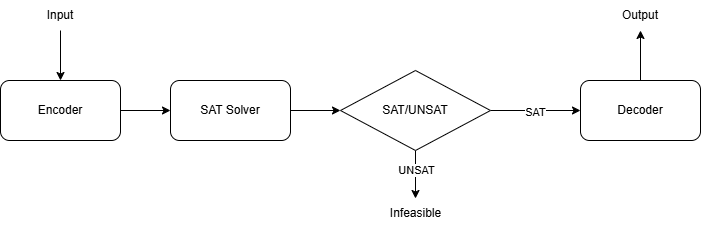
\includegraphics[width=0.75\linewidth]{figures/sat_flow.png}
    \caption{Sơ đồ luồng thực thi tổng thể của bộ giải SAT hiện đại (SAT Solver Execution Flow).}
    \label{fig:sat_flow}
\end{figure}

Như được mô tả trên Hình~\ref{fig:sat_flow}, quy trình giải quyết bài toán bắt đầu từ việc hình thức hóa bài toán thực tế thành các ràng buộc logic, mã hóa thành công thức CNF, chuyển vào bộ giải SAT và phân tích nghiệm trả về.

Thuật toán hiện đại nhất được áp dụng trong các SAT solver (như Glucose4, MiniSat, Lingeling) là thuật toán \textbf{Học Mệnh đề theo Xung đột (Conflict-Driven Clause Learning - CDCL)} \cite{moskewicz2001chaff,audemard2009predicting,biere2010lingeling}. CDCL nâng cấp thuật toán DPLL cổ điển nhờ các trụ cột công nghệ:
\begin{enumerate}
    \item \textbf{Lan truyền đơn vị (Unit Propagation - UP) và Two-Watched Literals (2WL):} Cơ chế theo dõi đúng hai literal chưa gán trong mỗi mệnh đề giúp kiểm tra lan truyền trong thời gian $O(1)$ mà không cần duyệt toàn bộ mệnh đề.
    \item \textbf{Phân tích xung đột và sinh mệnh đề học (Learnt Clause):} Khi một phép gán dẫn tới xung đột (tất cả literal trong mệnh đề đều $\mathbf{False}$), thuật toán lần ngược đồ thị hàm ý (Implication Graph) về điểm cắt First-UIP (Unique Implication Point) để sinh ra mệnh đề học, ngăn chặn không gian xung đột lặp lại trong tương lai.
    \item \textbf{Nhảy ngược phi tuần tự (Non-chronological Backjumping):} Nhảy ngược nhiều mức quyết định về mức an toàn cao hơn ngay sau xung đột.
    \item \textbf{Heuristic rẽ nhánh VSIDS (Variable State Independent Decaying Sum):} Ưu tiên chọn biến rẽ nhánh có tần suất tham gia vào các xung đột gần đây nhất, với trọng số suy giảm theo hàm mũ.
    \item \textbf{Thu dọn mệnh đề học dựa trên LBD (Literal Block Distance):} Đo đạc chất lượng của mệnh đề học dựa trên số mức quyết định phân biệt xuất hiện trong mệnh đề; các mệnh đề có LBD nhỏ được lưu trữ vĩnh viễn nhằm tối ưu bộ nhớ cache \cite{audemard2009predicting}.
\end{enumerate}

\section{Mã hóa dựa trên SAT (SAT-based Encoding)}
\label{sec:sat_encoding_concept}
Mã hóa SAT là quá trình chuyển đổi một bài toán thỏa mãn ràng buộc cấp cao (CSP) thành một công thức CNF tương đương. Một kỹ thuật mã hóa tốt phải cân bằng hoàn hảo giữa:
\begin{itemize}
    \item \textbf{Số lượng mệnh đề CNF:} Giữ số mệnh đề ở mức tuyến tính hoặc gần tuyến tính để tránh cạn kiệt bộ nhớ RAM.
    \item \textbf{Số lượng biến phụ trợ (Auxiliary Variables):} Tránh tạo ra quá nhiều biến phụ vì sẽ mở rộng không gian tìm kiếm Boolean của thuật toán phân nhánh.
    \item \textbf{Tính bảo toàn Arc-Consistency (GAC):} Khả năng phát hiện và cắt tỉa các giá trị vi phạm trực tiếp thông qua lan truyền đơn vị (Unit Propagation) mà không cần rẽ nhánh sâu.
\end{itemize}

\section{Các phương pháp mã hóa tối ưu cho ràng buộc At-Most-One (AMO)}
\label{sec:amo_encodings}
Xét tập hợp $m$ biến $X = \{x_1, x_2, \dots, x_m\}$, ràng buộc At-Most-One yêu cầu $\sum_{i=1}^m x_i \le 1$. Bốn kỹ thuật mã hóa nâng cao được khảo sát bao gồm:

\subsection{Mã hóa Nhị phân (Binary / Bitwise Encoding)}
Ý tưởng của Frisch et al. \cite{frisch2005atmost} là mã hóa vị trí biến nhận giá trị $\mathbf{True}$ bằng một chuỗi bit nhị phân:
\begin{itemize}
    \item Cần $k = \lceil \log_2 m \rceil$ biến phụ $b_1, b_2, \dots, b_k$.
    \item Với mỗi biến $x_i$, gọi chuỗi biểu diễn nhị phân của $(i-1)$ là $d_1 d_2 \dots d_k \in \{0, 1\}^k$. Nếu $x_i$ nhận giá trị $\mathbf{True}$, thì vector biến phụ $(b_1, \dots, b_k)$ phải khớp chính xác với mã nhị phân này:
    \begin{equation}
    x_i \to \bigwedge_{j=1}^k (b_j = d_j) \iff \bigwedge_{j=1}^k (\neg x_i \lor l_{j, d_j})
    \end{equation}
    trong đó $l_{j, 1} = b_j$ và $l_{j, 0} = \neg b_j$.
    \item Số biến phụ: $O(\log m)$.
    \item Số mệnh đề: $m \lceil \log_2 m \rceil = O(m \log m)$.
\end{itemize}

\subsection{Mã hóa Bộ đếm Tuần tự (Sequential Counter Encoding)}
Được Carsten Sinz đề xuất năm 2005 \cite{sinz2005towards}, kỹ thuật này mô phỏng thanh ghi phần cứng tích lũy số lượng giá trị $\mathbf{True}$:
\begin{itemize}
    \item Sử dụng $m-1$ biến phụ $s_1, s_2, \dots, s_{m-1}$, trong đó $s_i$ biểu thị trạng thái "đã có ít nhất một biến trong tiền tố $\{x_1, \dots, x_i\}$ nhận giá trị $\mathbf{True}$".
    \item Hệ thống mệnh đề gồm:
    \begin{align}
    (\neg x_1 \lor s_1) & \\
    (\neg s_{i-1} \lor s_i) & \quad \forall i \in [2, m-1] \quad \text{(Truyền trạng thái)} \\
    (\neg x_i \lor s_i) & \quad \forall i \in [2, m-1] \quad \text{(Gán trạng thái)} \\
    (\neg s_{i-1} \lor \neg x_i) & \quad \forall i \in [2, m] \quad \text{(Cấm trùng lặp)}
    \end{align}
    \item Số biến phụ: $m - 1 = O(m)$.
    \item Số mệnh đề: $3m - 4 = O(m)$.
    \item Ưu điểm lý thuyết: Duy trì đầy đủ tính nhất quán cung tổng quát (GAC) qua lan truyền đơn vị.
\end{itemize}

\subsection{Mã hóa Biến chỉ huy (Commander Variable Encoding)}
Klieber và Kwon (2007) \cite{klieber2007commander} đề xuất chia tập biến $X$ thành các nhóm con nhỏ kích thước $g$ (thường chọn $g=3$):
\begin{itemize}
    \item Với mỗi nhóm $G_i$, ta giới thiệu một "biến chỉ huy" $c_i$. Biến $c_i = \mathbf{True}$ khi và chỉ khi có đúng một biến trong nhóm $G_i$ là $\mathbf{True}$.
    \item Trong từng nhóm con $G_i$, áp dụng mã hóa Pairwise cục bộ ($\binom{g}{2} = 3$ mệnh đề).
    \item Áp dụng ràng buộc AMO đệ quy trên tập các biến chỉ huy $\{c_1, c_2, \dots, c_{\lceil m/g \rceil}\}$.
    \item Số biến phụ: $O(m/g)$.
    \item Số mệnh đề: Tuyến tính $O(m)$.
\end{itemize}

\subsection{Mã hóa Ma trận 2-Product (Product Encoding)}
Jingchao Chen (2010) \cite{chen2010new} đề xuất ánh xạ tập $m$ biến vào một lưới ma trận hai chiều kích thước $p \times q$ sao cho $p \times q \ge m$ (với $p \approx q \approx \lceil \sqrt{m} \rceil$):
\begin{itemize}
    \item Mỗi biến $x_i$ được gán tọa độ $(u, v)$ duy nhất trên lưới ($1 \le u \le p, 1 \le v \le q$).
    \item Giới thiệu hai tập biến phụ: hàng $r_1, \dots, r_p$ và cột $c_1, \dots, c_q$.
    \item Nếu $x_i$ là $\mathbf{True}$, thì cả hàng $r_u$ và cột $c_v$ phải nhận $\mathbf{True}$:
    \begin{equation}
    x_i \to r_u \land c_v \iff (\neg x_i \lor r_u) \land (\neg x_i \lor c_v)
    \end{equation}
    \item Ràng buộc AMO trên tập hàng $\{r_1, \dots, r_p\}$ và tập cột $\{c_1, \dots, c_q\}$.
    \item Số biến phụ: $p + q = O(\sqrt{m})$.
    \item Số mệnh đề: $2m + O(p^2 + q^2) = O(m)$.
\end{itemize}

% =============================================================================
% CHƯƠNG 3: PHƯƠNG PHÁP ĐỀ XUẤT VÀ MÔ HÌNH HÓA
% =============================================================================
\chapter{Phương pháp đề xuất và Mô hình hóa}
\label{chap:methodology}

\section{Tổng quan về phương pháp tiếp cận}
\label{sec:method_overview}
Để đánh giá toàn diện năng lực giải quyết bài toán $N$-Queens, tôi triển khai hai trục nghiên cứu song song:
\begin{enumerate}
    \item \textbf{Trục 1 (SAT Solving):} Triển khai và đối chuẩn 5 kỹ thuật mã hóa ràng buộc AMO: Binomial (Pairwise), Binary, Sequential Counter, Commander Variable ($g=3$), và 2-Product trên cùng một SAT solver công nghiệp (PySAT Glucose4).
    \item \textbf{Trục 2 (So sánh Đa Mô hình - Cross-Paradigm):} Đối đầu trực diện giữa cấu hình SAT tối ưu nhất với hai trường phái tính toán chính xác đối chiếu: Lập trình Ràng buộc (Google OR-Tools CP-SAT, IBM ILOG CPLEX CP Optimizer) và Quy hoạch Tuyến tính Nguyên 0-1 (Gurobi MIP, IBM ILOG CPLEX MIP).
\end{enumerate}

\section{Ứng dụng các phương pháp mã hóa SAT cho N-Queens}
\label{sec:sat_encodings_nqueens}
Ma trận bàn cờ $N \times N$ gồm các biến nhị phân $B_{i,j}$ ($0 \le i, j < N$). Các ràng buộc được thiết lập cụ thể:

\subsection{Ràng buộc trên Hàng và Cột}
Mỗi hàng $i$ và mỗi cột $j$ có đúng một quân hậu:
\begin{align}
\text{ALO: } & \bigvee_{j=0}^{N-1} B_{i,j} \quad \forall i \in [0, N-1], \qquad \bigvee_{i=0}^{N-1} B_{i,j} \quad \forall j \in [0, N-1] \\
\text{AMO: } & \text{AMO}(B_{i,0}, \dots, B_{i,N-1}) \quad \forall i, \qquad \text{AMO}(B_{0,j}, \dots, B_{N-1,j}) \quad \forall j
\end{align}

\subsection{Ràng buộc trên Đường chéo}
Bàn cờ có $2N - 1$ đường chéo chính (chỉ số $k = i - j \in [-(N-1), N-1]$) và $2N - 1$ đường chéo phụ (chỉ số $k = i + j \in [0, 2N-2]$). Vì các đường chéo ở bốn góc chỉ chứa đúng 1 ô (không thể có xung đột), ta chỉ cần áp dụng AMO cho các đường chéo có độ dài $m \ge 2$:
\begin{align}
\text{Đường chéo chính: } & \text{AMO}(\{B_{i,j} \mid i - j = k\}), \quad \forall k \in [-(N-2), N-2] \\
\text{Đường chéo phụ: } & \text{AMO}(\{B_{i,j} \mid i + j = k\}), \quad \forall k \in [1, 2N-3]
\end{align}

\subsection{So sánh Độ phức tạp Lý thuyết giữa 5 SAT Encodings}
Bảng~\ref{tab:encoding_complexity} tổng hợp độ phức tạp tiệm cận của 5 phương pháp mã hóa trên một ràng buộc AMO có $m$ biến và trên toàn bộ bài toán $N$-Queens.

\begin{table}[htbp]
\centering
\small
\caption{So sánh độ phức tạp lý thuyết của 5 phương pháp mã hóa SAT trên bài toán $N$-Queens.}
\label{tab:encoding_complexity}
\begin{tabular}{lcccc}
\toprule
\textbf{Kỹ thuật Mã hóa} & \textbf{\shortstack{Biến phụ\\/ AMO}} & \textbf{\shortstack{Mệnh đề\\/ AMO}} & \textbf{\shortstack{Tổng\\mệnh đề}} & \textbf{\shortstack{Bảo toàn\\GAC}} \\
\midrule
\textbf{Binomial (Pairwise)} & $0$ & $O(m^2)$ & $O(N^4)$ & Có \\
\textbf{Sequential Counter}  & $O(m)$ & $O(m)$ & $O(N^2)$ & Có \\
\textbf{Binary (Bitwise)}    & $O(\log m)$ & $O(m \log m)$ & $O(N^2 \log N)$ & Không \\
\textbf{Commander Variable}  & $O(m/g)$ & $O(m)$ & $O(N^2)$ & Không \\
\textbf{2-Product}           & $O(\sqrt{m})$ & $O(m)$ & $O(N^2)$ & Không \\
\bottomrule
\end{tabular}
\end{table}

\section{Mô hình hóa Đa Trường phái (CP và MIP)}
\label{sec:cp_mip_formulations}

\subsection{Mô hình Lập trình Ràng buộc (Constraint Programming - CP)}
Trường phái CP mô tả bài toán một cách tự nhiên và cô đọng nhất bằng cách sử dụng $N$ biến nguyên $Q_0, Q_1, \dots, Q_{N-1}$ với miền giá trị $D(Q_i) = \{0, 1, \dots, N-1\}$, trong đó $Q_i$ biểu diễn chỉ số cột của quân hậu tại hàng $i$:
\begin{align}
\text{AllDifferent}(Q_0, Q_1, \dots, Q_{N-1}) & \quad \text{(Không trùng cột)} \\
\text{AllDifferent}(Q_0 + 0, Q_1 + 1, \dots, Q_{N-1} + (N-1)) & \quad \text{(Không trùng đường chéo phụ)} \\
\text{AllDifferent}(Q_0 - 0, Q_1 - 1, \dots, Q_{N-1} - (N-1)) & \quad \text{(Không trùng đường chéo chính)}
\end{align}
Toàn bộ bài toán quy mô $N$ bất kỳ chỉ cần đúng $N$ biến nguyên và đúng 3 ràng buộc toàn cục $\text{AllDifferent}$. Bộ giải IBM ILOG CPLEX CP Optimizer áp dụng thuật toán lan truyền Régin \cite{regin1994filtering} để lọc miền giá trị cực mạnh dựa trên bài toán tìm cặp ghép cực đại trên đồ thị hai phía.

\subsection{Mô hình Quy hoạch Tuyến tính Nguyên 0-1 (MIP / 0-1 ILP)}
Trường phái MIP mô hình hóa bài toán bằng $N^2$ biến nhị phân $x_{i,j} \in \{0, 1\}$ tương tự SAT:
\begin{align}
\sum_{j=0}^{N-1} x_{i,j} &= 1 \quad \forall i \in [0, N-1] \quad \text{(Mỗi hàng đúng 1 quân hậu)} \\
\sum_{i=0}^{N-1} x_{i,j} &= 1 \quad \forall j \in [0, N-1] \quad \text{(Mỗi cột đúng 1 quân hậu)} \\
\sum_{i-j=k} x_{i,j} &\le 1 \quad \forall k \in [-(N-2), N-2] \quad \text{(Đường chéo chính)} \\
\sum_{i+j=k} x_{i,j} &\le 1 \quad \forall k \in [1, 2N-3] \quad \text{(Đường chéo phụ)}
\end{align}
Mô hình chứa $N^2$ biến nhị phân và $6N - 6$ ràng buộc bất đẳng thức tuyến tính, được giải quyết bằng thuật toán Branch-and-Cut kết hợp mặt cắt đa diện và nới lỏng đơn hình (Simplex LP relaxation).

% =============================================================================
% CHƯƠNG 4: THỰC NGHIỆM VÀ ĐÁNH GIÁ KẾT QUẢ
% =============================================================================
\chapter{Thực nghiệm và Đánh giá kết quả}
\label{chap:experiments}

\section{Thiết lập không gian đo đạc và tập dữ liệu}
\label{sec:dataset_settings}
Để kiểm tra triệt để năng lực mở rộng (scalability) của các thuật toán, không gian thực nghiệm được thiết kế đồng bộ trên chuỗi 15 mốc kích thước:
\begin{equation}
N \in \{4, 8, 16, 25, 36, 49, 64, 81, 100, 125, 216, 343, 512, 729, 1000\}
\end{equation}
Mốc $N = 1000$ đại diện cho bài toán quy mô cực lớn với $1.000.000$ biến quyết định và xấp xỉ $14.000.000$ mệnh đề CNF.
Giới hạn thời gian (Timeout) được thiết lập nghiêm ngặt là \textbf{$120.0$ giây} cho mỗi lượt chạy. Nếu bộ giải không tìm được nghiệm trong thời gian này, kết quả được đánh dấu là \texttt{TIMEOUT}. Các mốc sinh mệnh đề vượt ngưỡng 16 GB RAM được gắn nhãn \texttt{SKIPPED\_MEMLIMIT} để bảo vệ hệ thống.

\section{Môi trường thực nghiệm}
\label{sec:exp_env}
Thông số chi tiết về phần cứng và phiên bản phần mềm được chuẩn hóa trong Bảng~\ref{tab:env_config}.

\begin{table}[htbp]
\centering
\caption{Cấu hình môi trường phần cứng và phần mềm thực nghiệm.}
\label{tab:env_config}
\begin{tabularx}{\textwidth}{>{\raggedright\arraybackslash}p{4.8cm} X}
\toprule
\textbf{Thông số} & \textbf{Chi tiết cấu hình} \\
\midrule
Bộ vi xử lý (CPU) & 12th Gen Intel(R) Core(TM) i5-14500H (12 cores, 8 threads, up to 4.4 GHz) \\
Bộ nhớ trong (RAM) & 16.0 GB DDR4 \\
Hệ điều hành & Ubuntu 26.04 LTS (Linux x86\_64) \\
Môi trường thực thi & Python 3.14.4 \\
Bộ giải SAT & PySAT v1.9.dev15 (Solver core: Glucose4) \\
Bộ giải CP (Engine lai) & Google OR-Tools v9.15.6755 (CP-SAT Solver) \\
Bộ giải CP (Engine thuần) & IBM ILOG CPLEX Optimization Studio v22.1.1 (CP Optimizer) \\
Bộ giải MIP 1 & Gurobi Optimizer v13.0.3 (Academic License) \\
Bộ giải MIP 2 & IBM ILOG CPLEX Optimization Studio v22.1.1 (MIP Academic License) \\
\bottomrule
\end{tabularx}
\end{table}

\section{Đánh giá so sánh giữa 5 kỹ thuật mã hóa SAT}
\label{sec:sat_enc_results}

Bảng~\ref{tab:sat_encodings_runtime} đối chiếu trực tiếp thời gian thực thi (giây) của 5 kỹ thuật mã hóa SAT trên bộ giải Glucose4 qua 15 mốc kích thước bàn cờ. Bảng số liệu chi tiết toàn diện về số biến và số mệnh đề được tổng hợp trong Phụ lục~\ref{app:detailed_data}.

\begin{table}[htbp]
\centering
\caption{Bảng thời gian thực thi (giây) của 5 kỹ thuật mã hóa SAT trên bộ giải Glucose4 qua 15 mốc kích thước ($N \in [4, 1000]$).}
\label{tab:sat_encodings_runtime}
\begin{tabular}{rrrrrr}
\toprule
$N$ & \textbf{Binomial} & \textbf{Binary} & \textbf{Sequential} & \textbf{Commander} & \textbf{2-Product} \\
\midrule
4    & 0.00039 & 0.00041 & 0.00032 & \textbf{0.00021} & 0.00034 \\
8    & 0.00079 & 0.00075 & 0.00077 & 0.00081 & \textbf{0.00072} \\
16   & 0.01094 & 0.02093 & \textbf{0.00600} & 0.01760 & 0.10392 \\
25   & \textbf{0.00916} & 0.05290 & 0.06090 & 0.17529 & 0.14078 \\
36   & \textbf{0.02714} & 0.05251 & 0.16478 & 0.04235 & 7.73743 \\
49   & 0.08398 & \textbf{0.05116} & 1.14570 & 0.83751 & 10.47424 \\
64   & 0.18140 & 0.13639 & 1.65263 & \textbf{0.06721} & 12.07009 \\
81   & 0.35869 & \textbf{0.11759} & 24.01935 & 0.27075 & 15.55798 \\
100  & 0.68852 & \textbf{0.14738} & 46.52458 & 0.16474 & 15.32860 \\
125  & 1.29502 & \textbf{0.24989} & 45.29085 & 0.61935 & 25.38504 \\
216  & 6.03935 & \textbf{0.81394} & 89.66358 & 1.29397 & 41.69153 \\
343  & 19.89517 & 2.31824 & \texttt{TIMEOUT} & \textbf{2.09605} & 69.55248 \\
512  & \texttt{MEMLIMIT} & \textbf{5.44507} & \texttt{TIMEOUT} & 6.67240 & \texttt{TIMEOUT} \\
729  & \texttt{MEMLIMIT} & 64.82834 & \texttt{TIMEOUT} & \textbf{28.44704} & \texttt{TIMEOUT} \\
1000 & \texttt{MEMLIMIT} & 24.66207 & \texttt{TIMEOUT} & \textbf{20.09668} & \texttt{TIMEOUT} \\
\bottomrule
\end{tabular}
\end{table}

\begin{figure}[htbp]
    \centering
    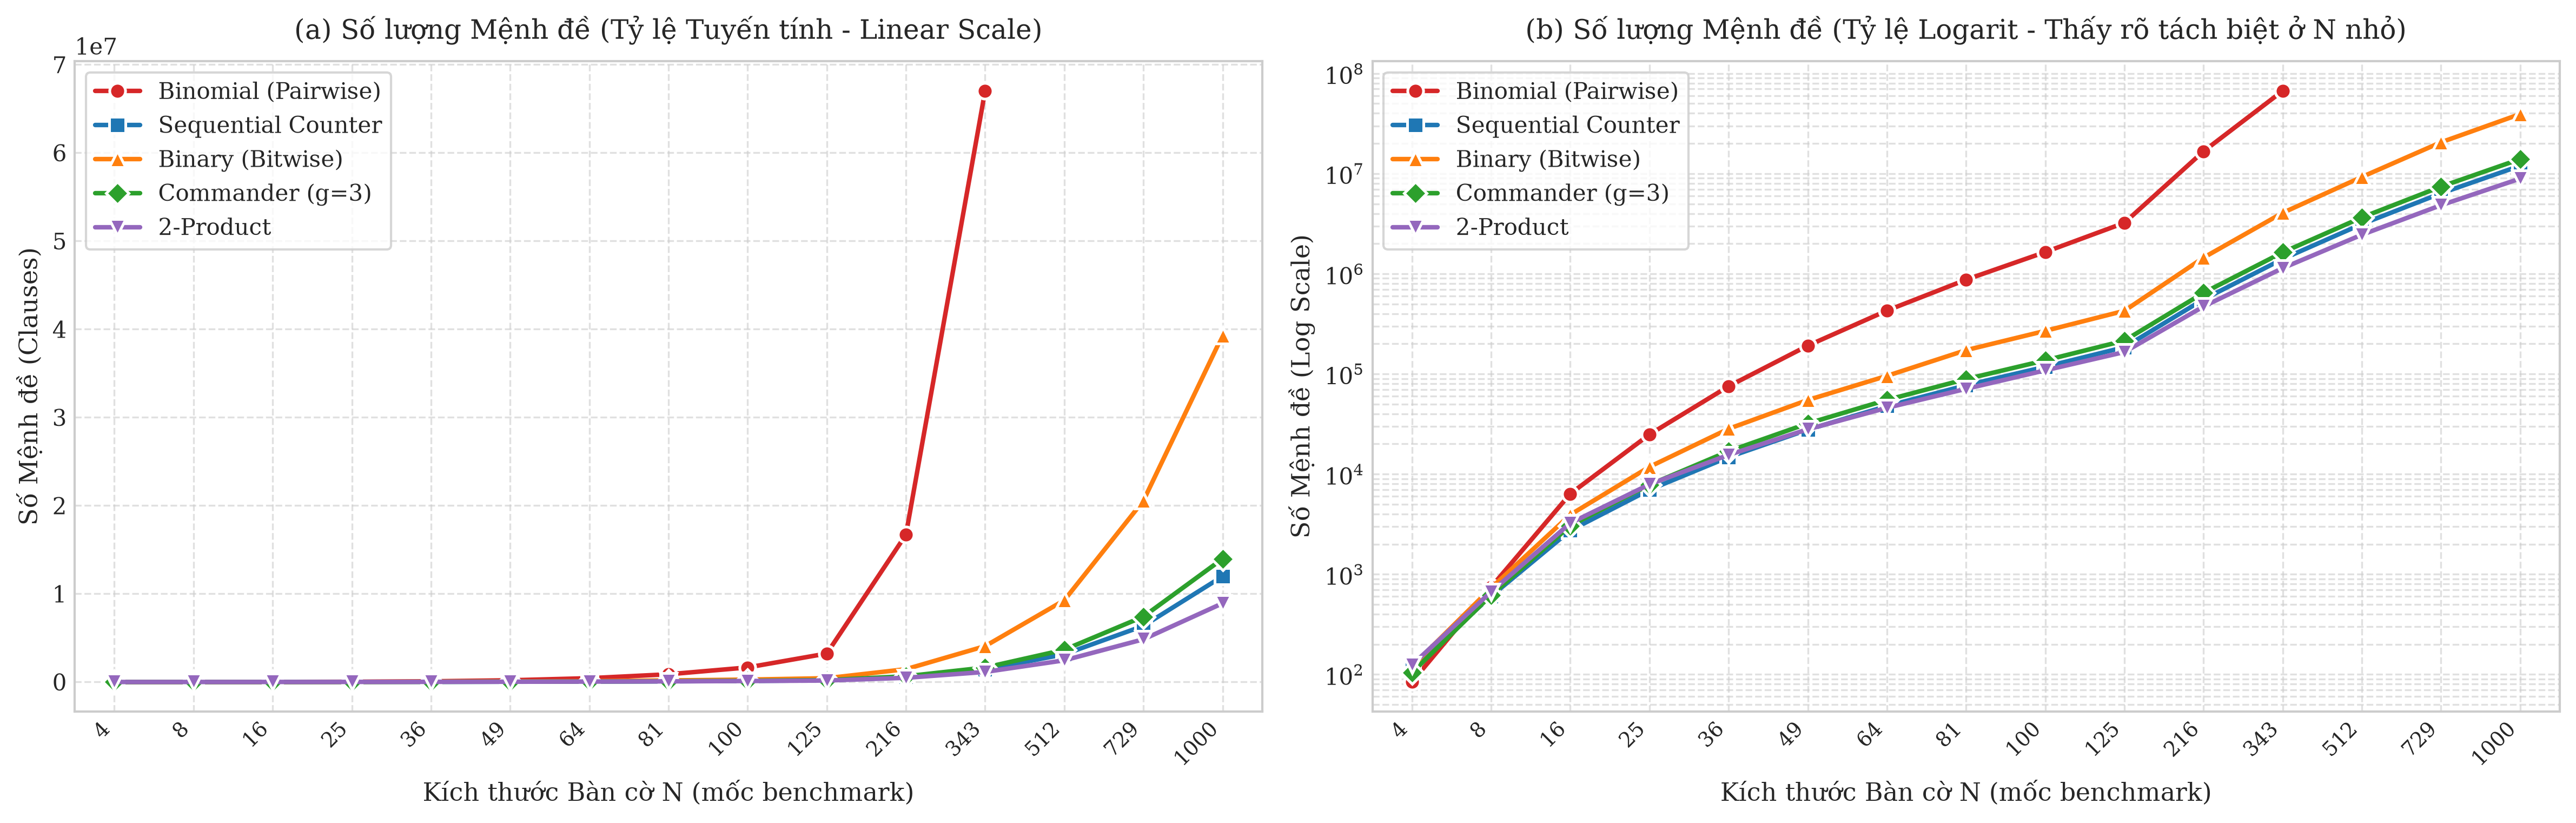
\includegraphics[width=0.95\linewidth]{figures/encoding_clauses.png}
    \caption{So sánh số lượng mệnh đề CNF sinh ra giữa 5 kỹ thuật mã hóa SAT qua 15 mốc kích thước ($N \in [4, 1000]$) trên thang tuyến tính (trái) và thang logarit (phải).}
    \label{fig:enc_clauses}
\end{figure}

\begin{figure}[htbp]
    \centering
    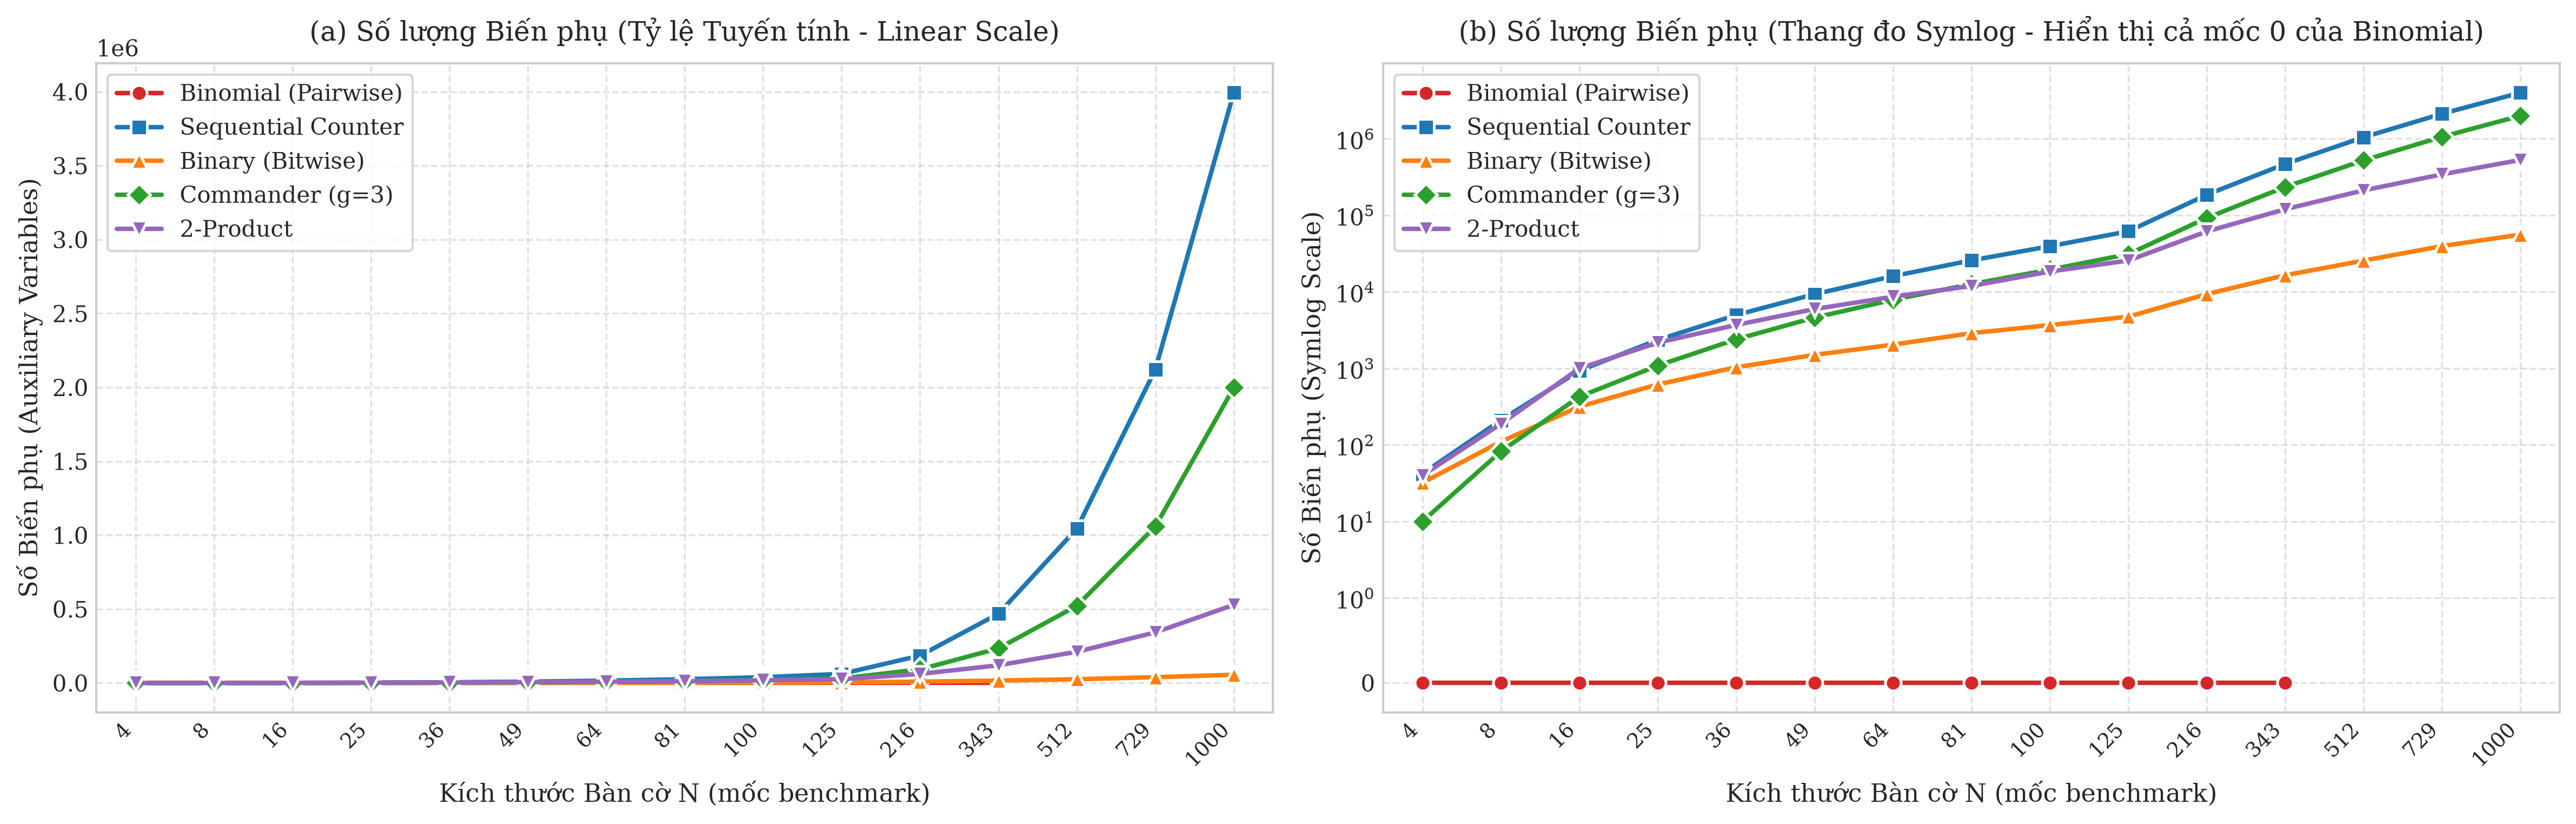
\includegraphics[width=0.95\linewidth]{figures/encoding_aux_vars.png}
    \caption{So sánh số lượng biến phụ trợ giữa 5 kỹ thuật mã hóa SAT qua 15 mốc kích thước ($N \in [4, 1000]$) trên thang tuyến tính (trái) và thang symlog (phải).}
    \label{fig:enc_aux_vars}
\end{figure}

\begin{figure}[htbp]
    \centering
    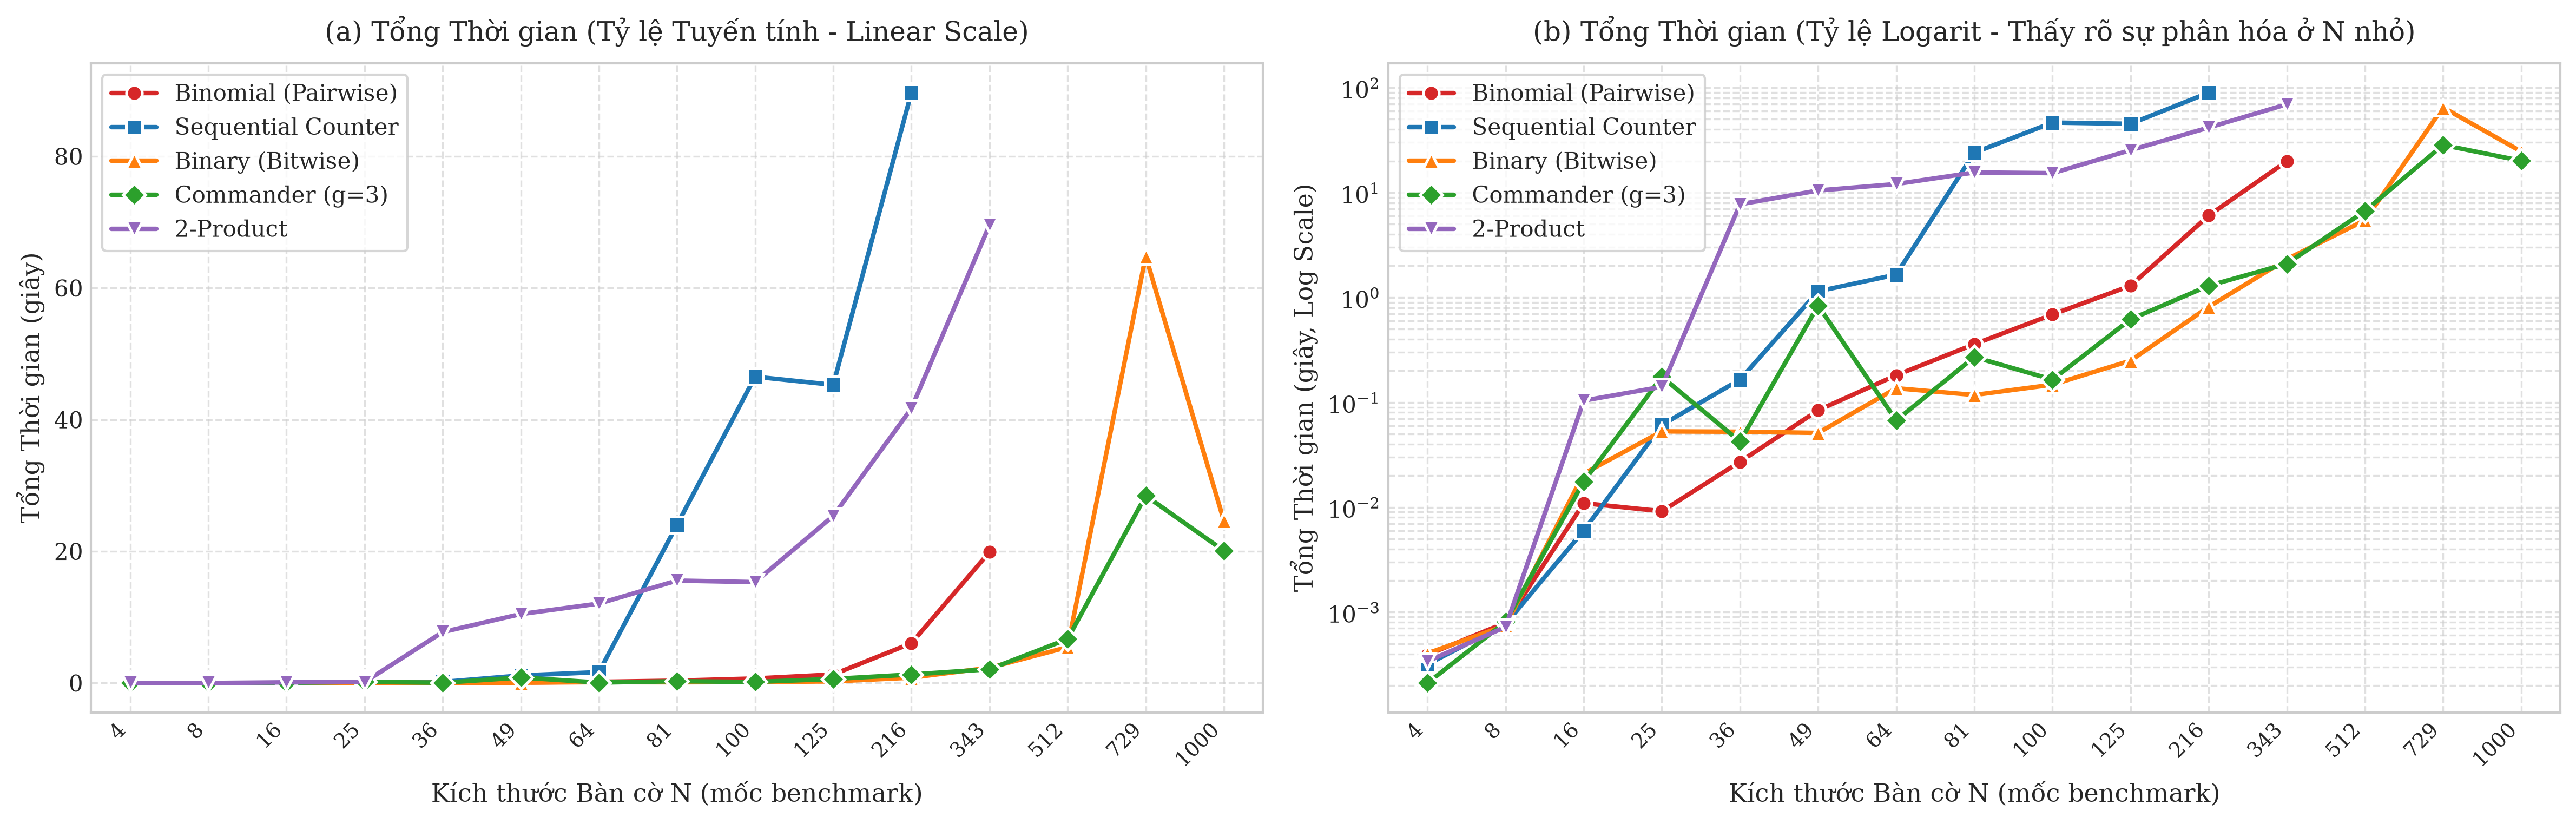
\includegraphics[width=0.95\linewidth]{figures/encoding_total_time.png}
    \caption{So sánh tổng thời gian thực thi giữa 5 kỹ thuật mã hóa SAT trên bộ giải Glucose4 qua 15 mốc kích thước ($N \in [4, 1000]$) trên thang tuyến tính (trái) và thang logarit (phải).}
    \label{fig:enc_time}
\end{figure}

\subsection{Phân tích Hiện tượng Bùng nổ Mệnh đề của Binomial}
Mã hóa Binomial thể hiện tốc độ giải cực nhanh ở các ma trận nhỏ ($N \le 25$) nhờ không sử dụng bất kỳ biến phụ nào ($0$ biến phụ). Tuy nhiên, số lượng mệnh đề tăng theo hàm bậc bốn $O(N^4)$ đã nhanh chóng bộc lộ giới hạn nghiêm trọng:
\begin{itemize}
    \item Tại $N = 100$, Binomial sinh ra hơn $1.64$ triệu mệnh đề.
    \item Tại $N = 343$, số mệnh đề vượt ngưỡng $67.0$ triệu mệnh đề, mất $5.09$ giây chỉ để sinh công thức và $14.80$ giây để giải.
    \item Tại $N \ge 512$, việc khởi tạo công thức đòi hỏi hơn 16 GB RAM, dẫn tới lỗi tràn bộ nhớ vật lý (\texttt{SKIPPED\_MEMLIMIT}).
\end{itemize}

\subsection{Nghịch lý Bộ đếm Tuần tự (Sequential Counter Paradox)}
Về mặt lý thuyết, Sequential Counter được coi là mô hình lý tưởng vì giữ số lượng mệnh đề ở mức tuyến tính $O(m)$ đồng thời bảo toàn trọn vẹn Arc-Consistency (GAC) qua lan truyền đơn vị \cite{sinz2005towards}. Thế nhưng, thực nghiệm lại chứng minh đây là kỹ thuật có hiệu năng kém nhất ở quy mô lớn, bị \texttt{TIMEOUT} ngay từ mốc $N = 343$.

Bản chất của nghịch lý này nằm ở sự xung đột nghiêm trọng giữa biến phụ và cơ chế phân nhánh của bộ giải CDCL:
\begin{enumerate}
    \item Tại $N = 1000$, Sequential Counter tạo ra tới $3.994.002$ biến phụ---gấp gần 4 lần số lượng biến quyết định ban đầu ($1.000.000$).
    \item Các mệnh đề truyền thanh ghi $(\neg s_{i-1} \lor s_i)$ tham gia dày đặc vào các chu trình lan truyền đơn vị và đồ thị hàm ý. Heuristic VSIDS liên tục cộng điểm hoạt động cho các biến thanh ghi phụ $s_i$, "đánh lừa" solver chọn các biến phụ này làm biến rẽ nhánh.
    \item Rẽ nhánh trên một biến tích lũy nội bộ $s_i$ có năng lực cắt tỉa không gian kém hơn rất nhiều so với rẽ nhánh trên biến bàn cờ gốc $B_{i,j}$, dẫn tới hiện tượng nghẽn tìm kiếm (search thrashing) và bùng nổ kích thước cây tìm kiếm.
\end{enumerate}

\subsection{Ưu thế Vượt trội của Binary và Commander Variable}
\begin{itemize}
    \item \textbf{Binary (Bitwise):} Tiết kiệm biến phụ nhất (chỉ $55.888$ biến phụ tại $N = 1000$, chiếm chưa đầy $5.6\%$ số biến gốc). Không gian biến được bảo toàn giúp heuristic VSIDS tập trung hoàn toàn vào biến quyết định bàn cờ, đạt tốc độ dẫn đầu trong phân khúc trung bình $N \in [49, 216]$ (chỉ $0.81$s tại $N=216$) và giải thành công toàn bộ 15 mốc lên đến $N = 1000$ trong $24.66$ giây.
    \item \textbf{Commander Variable ($g=3$):} Đạt điểm cân bằng lý tưởng nhất giữa việc giảm số lượng mệnh đề và kiểm soát số lượng biến phụ. Commander là kỹ thuật SAT nhanh nhất ở quy mô cực đại $N \ge 343$: hoàn thành $N = 343$ trong $2.10$s, $N = 729$ trong $28.45$s (nhanh hơn Binary $64.83$s gấp hơn 2 lần), và giải mốc $N = 1000$ chỉ trong $20.10$ giây.
\end{itemize}

\section{Thực nghiệm đối đầu Đa Mô hình (SAT vs CP vs MIP)}
\label{sec:cross_paradigm_results}

Bảng~\ref{tab:cross_paradigm_results} trình bày kết quả đối đầu trực diện giữa cấu hình SAT xuất sắc nhất (PySAT Glucose4 Commander) với 4 bộ giải công nghiệp thuộc trường phái CP và MIP qua 15 mốc kích thước.

\begin{table}[htbp]
\centering
\caption{Bảng đối đầu thực nghiệm thời gian thực thi (giây) giữa ba trường phái giải chính xác: SAT (Glucose4 Commander), Lập trình Ràng buộc CP (OR-Tools, CPLEX CP), và Quy hoạch Tuyến tính Nguyên MIP (Gurobi, CPLEX MIP) qua 15 mốc kích thước ($N \in [4, 1000]$).}
\label{tab:cross_paradigm_results}
\small
\setlength{\tabcolsep}{4pt}
\begin{tabular}{rrrrrr}
\toprule
$N$ & \textbf{\shortstack{PySAT\\(SAT)}} & \textbf{\shortstack{OR-Tools\\(CP)}} & \textbf{\shortstack{CPLEX\\(CP)}} & \textbf{\shortstack{Gurobi\\(MIP)}} & \textbf{\shortstack{CPLEX\\(MIP)}} \\
\midrule
4    & \textbf{0.00035} & 0.00693 & 0.01040 & 0.00144 & 0.02712 \\
8    & 0.00092 & 0.00484 & 0.00860 & \textbf{0.00075} & 0.01483 \\
16   & 0.01730 & 0.01142 & 0.00836 & \textbf{0.00782} & 0.01695 \\
25   & 0.17280 & 0.03455 & 0.01455 & \textbf{0.00247} & 0.02269 \\
36   & 0.03943 & 0.03944 & \textbf{0.01124} & 0.01598 & 0.03602 \\
49   & 0.81583 & 0.07143 & 0.01096 & \textbf{0.00850} & 0.04459 \\
64   & 0.06577 & 0.14754 & 0.01125 & \textbf{0.01115} & 0.07155 \\
81   & 0.28050 & 0.27732 & \textbf{0.01325} & 0.01780 & 0.09460 \\
100  & 0.17549 & 0.44541 & \textbf{0.01423} & 0.03066 & 0.12695 \\
125  & 0.66580 & 0.79482 & \textbf{0.01832} & 0.04310 & 0.20795 \\
216  & 1.27169 & 9.93486 & \textbf{0.02089} & 0.14242 & 0.66035 \\
343  & 2.13944 & 79.70357 & \textbf{0.03815} & 0.36060 & 1.94325 \\
512  & 6.29781 & \texttt{TIMEOUT} & \textbf{0.07285} & 0.83847 & 4.98140 \\
729  & 28.49975 & \texttt{TIMEOUT} & \textbf{0.12560} & 24.10297 & 14.90481 \\
1000 & 18.91856 & \texttt{TIMEOUT} & \textbf{0.25016} & \texttt{TIMEOUT} & 19.41587 \\
\bottomrule
\end{tabular}
\end{table}

\begin{figure}[htbp]
    \centering
    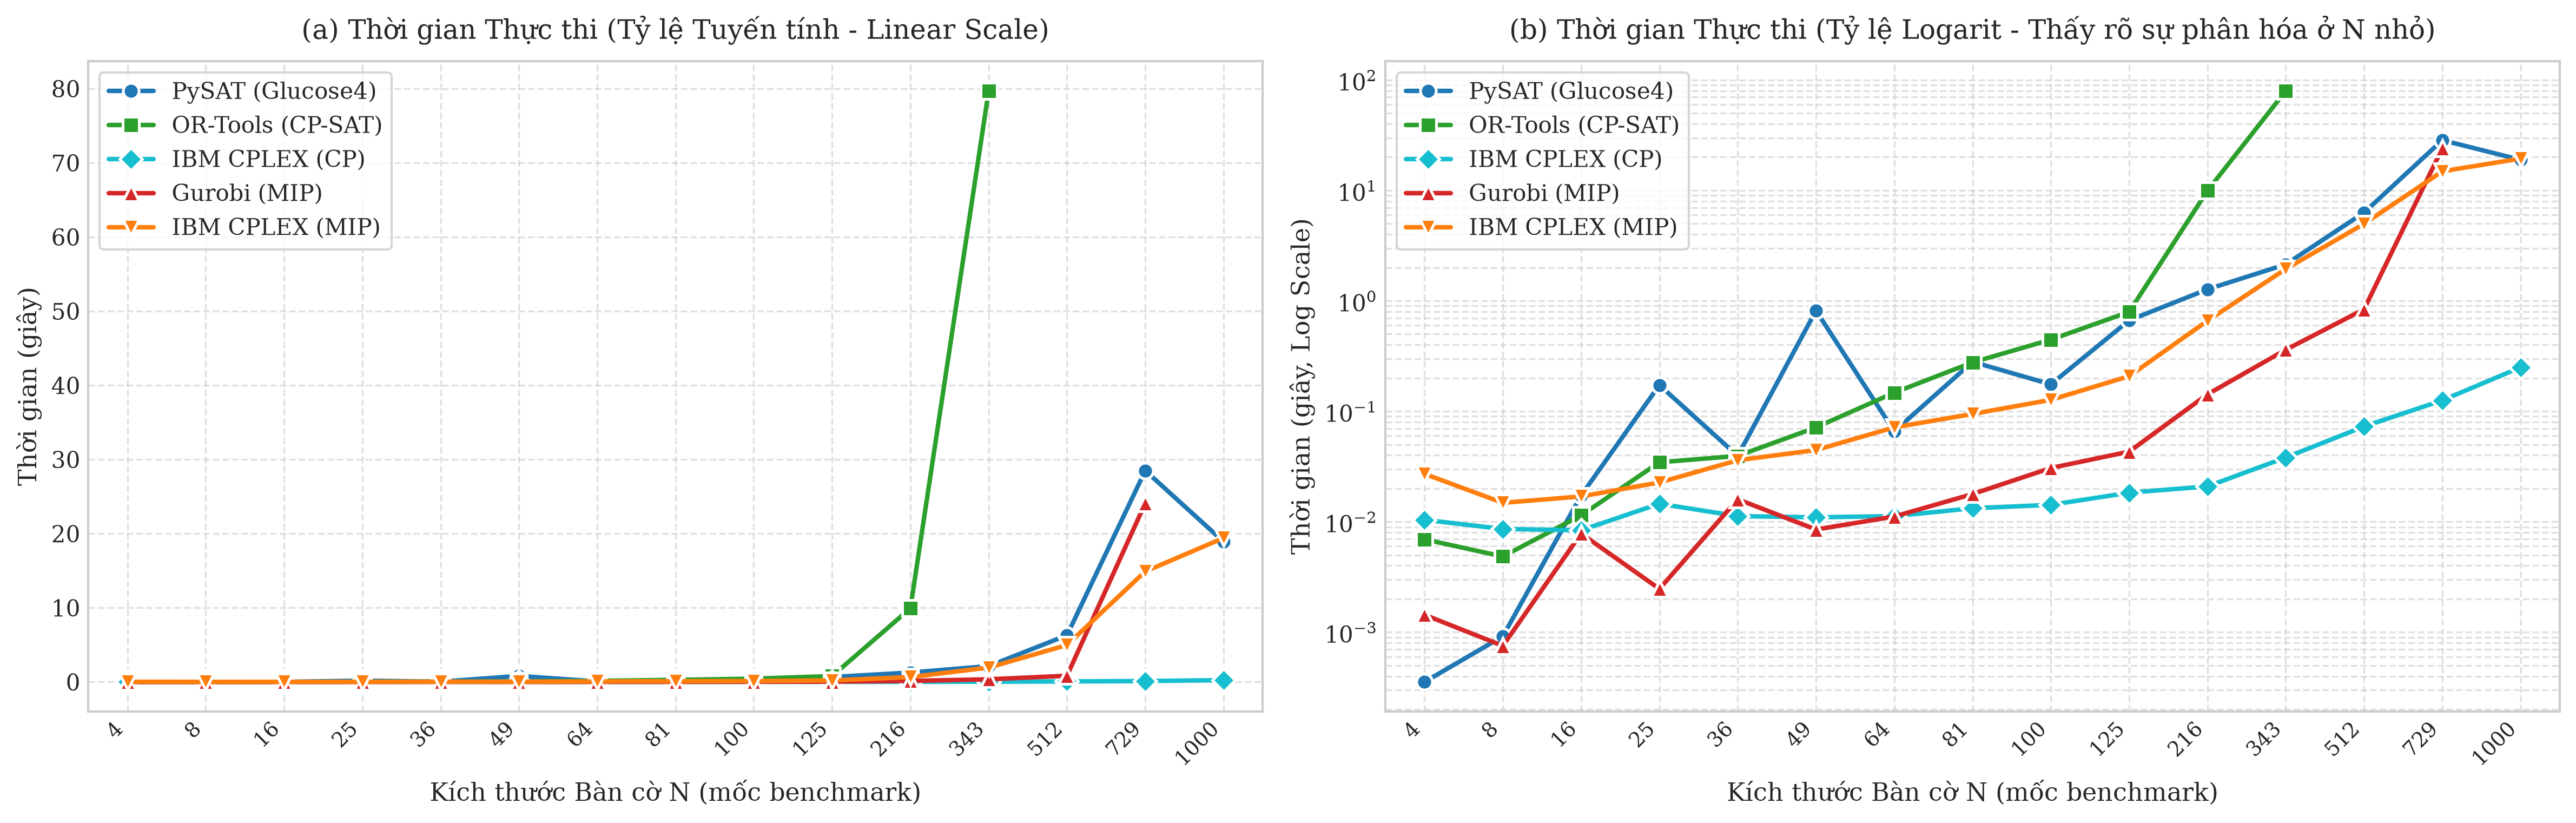
\includegraphics[width=0.95\linewidth]{figures/solver_total_time.png}
    \caption{So sánh thời gian thực thi đa mô hình (thang tuyến tính bên trái, thang logarit bên phải) giữa SAT (PySAT Glucose4 Commander), Lập trình ràng buộc CP (Google OR-Tools CP-SAT, IBM CPLEX CP), và Quy hoạch nguyên MIP (Gurobi MIP, IBM CPLEX MIP) qua 15 mốc kích thước ($N \in [4, 1000]$).}
    \label{fig:solver_time}
\end{figure}

\subsection{Thảo luận Chi tiết về Hiệu năng Đa Mô hình}
\begin{enumerate}
    \item \textbf{IBM CPLEX CP Optimizer:}
    Nhờ mô hình hóa chỉ với $N$ biến nguyên và 3 ràng buộc $\text{AllDifferent}$, kết hợp thuật toán lọc Régin dựa trên cặp ghép cực đại đồ thị hai phía, CPLEX CP duy trì thời gian giải dưới $0.04$ giây cho mọi $N \le 343$, và giải bàn cờ $N = 1000$ chỉ trong \textbf{$0.250$ giây}. Đây là giải pháp có hiệu năng áp đảo tuyệt đối cho bài toán N-Queens.
    
    \item \textbf{IBM CPLEX MIP:}
    Khi kích hoạt bản quyền học thuật đầy đủ, CPLEX MIP giải quyết thành công mốc $N = 1000$ ($1.000.000$ biến nhị phân) trong \textbf{$19.42$ giây}, chứng minh sức mạnh của thuật toán Presolve và các lát cắt đa diện Branch-and-Cut của IBM.
    
    \item \textbf{Gurobi Optimizer (MIP):}
    Gurobi đạt tốc độ cực nhanh: $N = 512$ ($262.144$ biến) trong $0.838$ giây, $N = 729$ ($531.441$ biến) trong $24.10$ giây. Tuy nhiên, tại $N = 1000$, không gian nhánh cận mở rộng khiến bộ giải chạm ngưỡng \texttt{TIMEOUT} (120s).
    
    \item \textbf{PySAT Glucose4 (Commander Variable):}
    Glucose4 với mã hóa Commander Variable giải thành công toàn bộ 15 mốc lên đến $N = 1000$ trong \textbf{$18.92$ giây} (ở benchmark solver) và $20.10$ giây (ở benchmark encoding). Đáng chú ý, Glucose4 đã vượt qua cả Gurobi lẫn OR-Tools CP-SAT tại mốc $N = 1000$, khẳng định rằng SAT CDCL hiện đại hoàn toàn đủ sức giải quyết bài toán hàng triệu biến Boolean khi được trang bị kỹ thuật mã hóa tối ưu.
    
    \item \textbf{Google OR-Tools (CP-SAT):}
    Đạt hiệu năng rất tốt ở $N \le 343$ ($79.70$ giây), nhưng chạm ngưỡng \texttt{TIMEOUT} tại $N \ge 512$ do kiến trúc phân rã (flattening) các ràng buộc toàn cục thành các mệnh đề giả Boolean nội bộ gặp quá tải tương tự Sequential Counter.
\end{enumerate}

% =============================================================================
% CHƯƠNG 5: KẾT LUẬN
% =============================================================================
\chapter{Kết luận}
\label{chap:conclusion}

\section{Đúc kết kết quả nghiên cứu}
\label{sec:conclusion_summary}
Báo cáo đã thực hiện một nghiên cứu thực nghiệm và lý thuyết chuyên sâu, toàn diện về bài toán $N$-Queens:
\begin{enumerate}
    \item Đánh giá chi tiết 5 kỹ thuật mã hóa At-Most-One (AMO) trong SAT: Chỉ ra bản chất hiện tượng bùng nổ mệnh đề bậc bốn của Binomial dẫn tới tràn bộ nhớ RAM ở $N \ge 512$, và làm sáng tỏ \textit{Nghịch lý Sequential Counter} khi sự bùng nổ hàng triệu biến phụ làm loãng heuristic phân nhánh VSIDS của thuật toán CDCL.
    \item Chứng minh sự vượt trội của mã hóa \textbf{Binary} trong việc tiết kiệm biến phụ ($55.9\text{K}$ biến tại $N=1000$, nhanh nhất ở $N \in [49, 216]$) và tính cân bằng hoàn hảo của mã hóa \textbf{Commander Variable} (nhanh nhất ở $N \ge 343$, giải $N = 1000$ trong $18.92$s).
    \item Khảo sát đối chuẩn liên trường phái (Cross-Paradigm Benchmark) giữa SAT, CP và MIP trên chuỗi 15 mốc kích thước đồng bộ lên tới $N = 1000$.
\end{enumerate}

\section{Khuyến nghị lựa chọn công nghệ giải}
\label{sec:recommendations}
Dựa trên các phân tích định lượng thực nghiệm, chúng tôi đưa ra khuyến nghị lựa chọn công cụ:
\begin{itemize}
    \item \textbf{Với bài toán thỏa mãn ràng buộc thuần túy quy mô cực đại ($N \ge 500$):} \textbf{Constraint Programming (IBM CPLEX CP Optimizer)} là giải pháp số một với tốc độ phản hồi tính bằng mili-giây ($0.25\text{s}$ cho $N = 1000$).
    \item \textbf{Với bài toán mô hình hóa nhị phân (0-1 Boolean formulation):} \textbf{PySAT Glucose4 (Commander Variable)} và \textbf{IBM CPLEX MIP} là hai đại diện xuất sắc nhất, đủ sức giải quyết bài toán chứa hàng triệu biến trong vòng 20 giây mà không gặp rào cản bộ nhớ.
\end{itemize}

\section*{Data Availability}
\addcontentsline{toc}{section}{Data Availability}
Toàn bộ mã nguồn cài đặt các thuật toán (5 kỹ thuật mã hóa SAT, 4 mô hình đối sánh CP và MIP), các kịch bản đo đạc tự động hóa thực nghiệm (benchmarks), tập dữ liệu kết quả đo đạc chi tiết (dạng CSV) và các biểu đồ phân tích trực quan hóa được công khai tại kho lưu trữ (Repository) của dự án:
\begin{center}
    \textbf{GitHub Repository:} \url{https://github.com/NhHung07/N_Queens.git}
\end{center}

% -----------------------------------------------------------------------------
% TÀI LIỆU THAM KHẢO (BIBLIOGRAPHY)
% -----------------------------------------------------------------------------
\begin{thebibliography}{99}
\addcontentsline{toc}{chapter}{Tài liệu tham khảo}

\bibitem{bezzel1848}
M.~Bezzel, Schachfreund, Berliner Schachzeitung 3 (1848) 363.

\bibitem{nauck1850}
F.~Nauck, Briefwechsel mit allen f{\"u}r alle, Illustrirte Zeitung 15 (377) (1850) 182.

\bibitem{letavec2002nqueens}
C.~Letavec, J.~Ruggiero, The n-queens problem, INFORMS Transactions on Education 2~(3) (2002) 101--103.

\bibitem{rivin1994nqueens}
I.~Rivin, I.~Vardi, P.~Zimmermann, The n-queens problem, The American Mathematical Monthly 101~(7) (1994) 629--639.

\bibitem{clarke1996formal}
E.~M. Clarke, J.~M. Wing, Formal methods: State of the art and future directions, ACM Computing Surveys 28~(4) (1996) 626--643.

\bibitem{barber2003introduction}
F.~Barber, M.~A. Salido, Introduction to constraint programming, Inteligencia Artificial, Revista Iberoamericana de Inteligencia Artificial 20 (2003) 13--30.

\bibitem{cook1971complexity}
S.~A. Cook, The complexity of theorem-proving procedures, in: Proceedings of the Third Annual ACM Symposium on Theory of Computing (STOC'71), ACM, 1971, pp. 151--158.

\bibitem{marques2008practical}
J.~Marques-Silva, Practical applications of boolean satisfiability, in: 2008 9th International Workshop on Discrete Event Systems, IEEE, 2008, pp. 74--80.

\bibitem{biere2009handbook}
A.~Biere, M.~Heule, H.~van Maaren, T.~Walsh (Eds.), Handbook of Satisfiability, Vol. 185, IOS Press, Amsterdam, 2009.

\bibitem{sosic1994polynomial}
R.~Sosic, J.~Gu, Efficient local search with conflict minimization: A polynomial-time algorithm for the n-queens problem, IEEE Transactions on Knowledge and Data Engineering 6~(5) (1994) 661--668.

\bibitem{erbas1992queens}
C.~Erbas, M.~M. Tanik, Generating solutions to the n-queens problem using 2-circulant matrices, Computers \& Mathematics with Applications 24~(11) (1992) 89--97.

\bibitem{hoffman2013traveling}
K.~L. Hoffman, M.~Padberg, G.~Rinaldi, Traveling salesman problem, Encyclopedia of Operations Research and Management Science 1 (2013) 1573--1578.

\bibitem{golomb1965backtrack}
S.~W. Golomb, L.~D. Baumert, Backtrack programming, Journal of the ACM 12~(4) (1965) 516--524.

\bibitem{bitner1975backtrack}
J.~R. Bitner, E.~M. Reingold, Backtrack programming techniques, Communications of the ACM 18~(11) (1975) 651--656.

\bibitem{simon2020reasoning}
L.~Simon, Reasoning with propositional logic: From sat solvers to knowledge compilation, A Guided Tour of Artificial Intelligence Research: Volume II (2020) 115--152.

\bibitem{moskewicz2001chaff}
M.~W. Moskewicz, C.~F. Madigan, Y.~Zhao, L.~Zhang, S.~Malik, Chaff: Accelerating engineering SAT runtimes, in: Proceedings of the 38th Design Automation Conference (DAC'01), ACM, 2001, pp. 530--535.

\bibitem{audemard2009predicting}
G.~Audemard, L.~Simon, Predicting learnt clauses quality in modern SAT solvers, in: Proceedings of the 21st International Joint Conference on Artificial Intelligence (IJCAI'09), 2009, pp. 399--404.

\bibitem{biere2010lingeling}
A.~Biere, Lingeling, plingeling, picosat and precosat at sat race 2010, FMV Report Series Technical Report 10/1, Johannes Kepler University, 2010.

\bibitem{sinz2005towards}
C.~Sinz, Towards an optimal CNF encoding of boolean cardinality constraints, in: Principles and Practice of Constraint Programming (CP 2005), Vol. 3709 of LNCS, Springer, 2005, pp. 827--831.

\bibitem{klieber2007commander}
W.~Klieber, G.~Kwon, Efficient CNF encoding for selecting at most one item from a group, in: Proceedings of the International Workshop on Constraints in Formal Verification (CFV'07), 2007, pp. 1--9.

\bibitem{chen2010new}
J.~Chen, A new SAT encoding of the at-most-one constraint, in: Proceedings of the 10th International Conference on Formal Methods in Computer-Aided Design (FMCAD'10), 2010, pp. 268--275.

\bibitem{frisch2005atmost}
A.~M. Frisch, P.~A. Giannaros, SAT encodings of the at-most-k constraint, in: Proceedings of the 3rd International Workshop on Modelling and Reformulating CSPs, 2005, pp. 45--56.

\bibitem{regin1994filtering}
J.-C. R{\'e}gin, A filtering algorithm for constraints of difference in CSPs, in: Proceedings of the 12th National Conference on Artificial Intelligence (AAAI'94), AAAI Press, 1994, pp. 362--367.

\end{thebibliography}

% -----------------------------------------------------------------------------
% PHỤ LỤC (APPENDIX)
% -----------------------------------------------------------------------------
\appendix
\chapter{Bảng số liệu chi tiết toàn diện của 5 Kỹ thuật SAT Encodings}
\label{app:detailed_data}

Dưới đây là toàn bộ số liệu đo đạc thực nghiệm chi tiết của 5 kỹ thuật mã hóa At-Most-One (AMO) trên bộ giải PySAT Glucose4 qua 15 mốc kích thước bàn cờ ($N \in [4, 1000]$).

\begingroup
\singlespacing
\scriptsize
\setlength{\tabcolsep}{2.5pt}
\begin{longtable}{r l r r r r r r c}
\caption{Toàn bộ số liệu đo đạc thực nghiệm 5 kỹ thuật mã hóa SAT trên PySAT Glucose4 qua 15 mốc kích thước.} \label{tab:full_sat_data} \\
\toprule
$N$ & \textbf{Kỹ thuật} & \textbf{\shortstack{Tổng\\biến}} & \textbf{\shortstack{Biến\\phụ}} & \textbf{\shortstack{Số\\mệnh đề}} & \textbf{\shortstack{TG sinh\\(s)}} & \textbf{\shortstack{TG giải\\(s)}} & \textbf{\shortstack{Tổng cộng\\(s)}} & \textbf{\shortstack{Trạng\\thái}} \\
\midrule
\endfirsthead

\multicolumn{9}{c}{\tablename\ \thetable\ -- tiếp theo từ trang trước} \\
\toprule
$N$ & \textbf{Kỹ thuật} & \textbf{\shortstack{Tổng\\biến}} & \textbf{\shortstack{Biến\\phụ}} & \textbf{\shortstack{Số\\mệnh đề}} & \textbf{\shortstack{TG sinh\\(s)}} & \textbf{\shortstack{TG giải\\(s)}} & \textbf{\shortstack{Tổng cộng\\(s)}} & \textbf{\shortstack{Trạng\\thái}} \\
\midrule
\endhead

\midrule
\multicolumn{9}{r}{Còn tiếp ở trang sau \dots} \\
\bottomrule
\endfoot

\bottomrule
\endlastfoot

\multirow{5}{*}{4} 
 & Binomial & 16 & 0 & 84 & 0.000031 & 0.000361 & 0.000393 & \texttt{SAT} \\
 & Sequential & 58 & 42 & 116 & 0.000033 & 0.000285 & 0.000318 & \texttt{SAT} \\
 & Binary & 48 & 32 & 120 & 0.000065 & 0.000339 & 0.000405 & \texttt{SAT} \\
 & Commander & 26 & 10 & 104 & 0.000040 & 0.000171 & \textbf{0.000211} & \texttt{SAT} \\
 & 2-Product & 56 & 40 & 124 & 0.000059 & 0.000281 & 0.000340 & \texttt{SAT} \\
\midrule
\multirow{5}{*}{8} 
 & Binomial & 64 & 0 & 744 & 0.000171 & 0.000622 & 0.000792 & \texttt{SAT} \\
 & Sequential & 274 & 210 & 604 & 0.000089 & 0.000684 & 0.000773 & \texttt{SAT} \\
 & Binary & 174 & 110 & 728 & 0.000144 & 0.000603 & 0.000746 & \texttt{SAT} \\
 & Commander & 146 & 82 & 618 & 0.000122 & 0.000686 & 0.000808 & \texttt{SAT} \\
 & 2-Product & 252 & 188 & 668 & 0.000109 & 0.000614 & \textbf{0.000723} & \texttt{SAT} \\
\midrule
\multirow{5}{*}{16} 
 & Binomial & 256 & 0 & 6,352 & 0.000570 & 0.010369 & 0.010939 & \texttt{SAT} \\
 & Sequential & 1,186 & 930 & 2,732 & 0.000194 & 0.005807 & \textbf{0.006000} & \texttt{SAT} \\
 & Binary & 572 & 316 & 3,928 & 0.000453 & 0.020475 & 0.020928 & \texttt{SAT} \\
 & Commander & 682 & 426 & 3,052 & 0.000424 & 0.017172 & 0.017596 & \texttt{SAT} \\
 & 2-Product & 1,252 & 996 & 3,236 & 0.000426 & 0.103495 & 0.103921 & \texttt{SAT} \\
\midrule
\multirow{5}{*}{25} 
 & Binomial & 625 & 0 & 24,850 & 0.001967 & 0.007194 & \textbf{0.009161} & \texttt{SAT} \\
 & Sequential & 2,977 & 2,352 & 6,962 & 0.000503 & 0.060392 & 0.060895 & \texttt{SAT} \\
 & Binary & 1,241 & 616 & 11,806 & 0.001082 & 0.051813 & 0.052895 & \texttt{SAT} \\
 & Commander & 1,709 & 1,084 & 7,810 & 0.001046 & 0.174248 & 0.175294 & \texttt{SAT} \\
 & 2-Product & 2,789 & 2,164 & 7,894 & 0.000722 & 0.140053 & 0.140775 & \texttt{SAT} \\
\midrule
\multirow{5}{*}{36} 
 & Binomial & 1,296 & 0 & 75,252 & 0.006442 & 0.020699 & \textbf{0.027140} & \texttt{SAT} \\
 & Sequential & 6,266 & 4,970 & 14,772 & 0.001122 & 0.163660 & 0.164782 & \texttt{SAT} \\
 & Binary & 2,328 & 1,032 & 28,320 & 0.002558 & 0.049948 & 0.052506 & \texttt{SAT} \\
 & Commander & 3,690 & 2,394 & 16,904 & 0.002307 & 0.040042 & 0.042349 & \texttt{SAT} \\
 & 2-Product & 4,988 & 3,692 & 15,548 & 0.001730 & 7.735702 & 7.737431 & \texttt{SAT} \\
\midrule
\multirow{5}{*}{49} 
 & Binomial & 2,401 & 0 & 191,394 & 0.030131 & 0.053853 & 0.083984 & \texttt{SAT} \\
 & Sequential & 11,713 & 9,312 & 27,746 & 0.012348 & 1.133353 & 1.145701 & \texttt{SAT} \\
 & Binary & 3,901 & 1,500 & 54,866 & 0.005207 & 0.045954 & \textbf{0.051161} & \texttt{SAT} \\
 & Commander & 7,009 & 4,608 & 32,014 & 0.003766 & 0.833742 & 0.837507 & \texttt{SAT} \\
 & 2-Product & 8,353 & 5,952 & 27,998 & 0.002204 & 10.472035 & 10.474239 & \texttt{SAT} \\
\midrule
\multirow{5}{*}{64} 
 & Binomial & 4,096 & 0 & 428,864 & 0.068978 & 0.112422 & 0.181400 & \texttt{SAT} \\
 & Sequential & 20,098 & 16,002 & 47,756 & 0.002972 & 1.649655 & 1.652627 & \texttt{SAT} \\
 & Binary & 6,136 & 2,040 & 95,576 & 0.011644 & 0.124750 & 0.136394 & \texttt{SAT} \\
 & Commander & 11,958 & 7,862 & 55,022 & 0.014461 & 0.052746 & \textbf{0.067207} & \texttt{SAT} \\
 & 2-Product & 12,732 & 8,636 & 45,876 & 0.003465 & 12.066623 & 12.070088 & \texttt{SAT} \\
\midrule
\multirow{5}{*}{81} 
 & Binomial & 6,561 & 0 & 872,802 & 0.149942 & 0.208745 & 0.358687 & \texttt{SAT} \\
 & Sequential & 32,321 & 25,760 & 76,962 & 0.005572 & 24.013778 & 24.019350 & \texttt{SAT} \\
 & Binary & 9,441 & 2,880 & 172,694 & 0.034938 & 0.082653 & \textbf{0.117590} & \texttt{SAT} \\
 & Commander & 19,177 & 12,616 & 88,778 & 0.013516 & 0.257236 & 0.270753 & \texttt{SAT} \\
 & 2-Product & 18,477 & 11,916 & 70,966 & 0.015049 & 15.542931 & 15.557980 & \texttt{SAT} \\
\midrule
\multirow{5}{*}{100} 
 & Binomial & 10,000 & 0 & 1,646,900 & 0.300462 & 0.388057 & 0.688519 & \texttt{SAT} \\
 & Sequential & 49,402 & 39,402 & 117,812 & 0.011384 & 46.513192 & 46.524576 & \texttt{SAT} \\
 & Binary & 13,678 & 3,678 & 269,024 & 0.051690 & 0.095692 & \textbf{0.147383} & \texttt{SAT} \\
 & Commander & 29,502 & 19,502 & 136,560 & 0.030482 & 0.134258 & 0.164740 & \texttt{SAT} \\
 & 2-Product & 28,408 & 18,408 & 108,596 & 0.010247 & 15.318352 & 15.328598 & \texttt{SAT} \\
\midrule
\multirow{5}{*}{125} 
 & Binomial & 15,625 & 0 & 3,224,250 & 0.509696 & 0.785323 & 1.295019 & \texttt{SAT} \\
 & Sequential & 77,377 & 61,752 & 184,762 & 0.024211 & 45.266639 & 45.290850 & \texttt{SAT} \\
 & Binary & 20,353 & 4,728 & 426,574 & 0.078129 & 0.171765 & \textbf{0.249894} & \texttt{SAT} \\
 & Commander & 46,685 & 31,060 & 214,918 & 0.041198 & 0.578150 & 0.619348 & \texttt{SAT} \\
 & 2-Product & 41,253 & 25,628 & 165,386 & 0.017037 & 25.367998 & 25.385035 & \texttt{SAT} \\
\midrule
\multirow{5}{*}{216} 
 & Binomial & 46,656 & 0 & 16,703,352 & 2.188771 & 3.850577 & 6.039348 & \texttt{SAT} \\
 & Sequential & 231,986 & 185,330 & 555,132 & 0.108629 & 89.554950 & 89.663579 & \texttt{SAT} \\
 & Binary & 55,988 & 9,332 & 1,449,224 & 0.278691 & 0.535247 & \textbf{0.813938} & \texttt{SAT} \\
 & Commander & 139,002 & 92,346 & 645,382 & 0.161277 & 1.132691 & 1.293968 & \texttt{SAT} \\
 & 2-Product & 108,096 & 61,440 & 471,448 & 0.060232 & 41.631297 & 41.691528 & \texttt{SAT} \\
\midrule
\multirow{5}{*}{343} 
 & Binomial & 117,649 & 0 & 67,021,514 & 5.093746 & 14.801421 & 19.895166 & \texttt{SAT} \\
 & Sequential & 586,189 & 468,540 & 1,404,254 & 0.227117 & - & - & \texttt{TIMEOUT} \\
 & Binary & 134,109 & 16,460 & 4,060,266 & 0.771659 & 1.546584 & 2.318243 & \texttt{SAT} \\
 & Commander & 351,857 & 234,208 & 1,635,926 & 0.304408 & 1.791643 & \textbf{2.096051} & \texttt{SAT} \\
 & 2-Product & 237,765 & 120,116 & 1,138,710 & 0.162234 & 69.390242 & 69.552476 & \texttt{SAT} \\
\midrule
\multirow{5}{*}{512} 
 & Binomial & 262,144 & 0 & - & - & - & - & \texttt{MEMLIMIT} \\
 & Sequential & 1,307,650 & 1,045,506 & 3,134,476 & 0.495823 & - & - & \texttt{TIMEOUT} \\
 & Binary & 287,730 & 25,586 & 9,262,424 & 1.613264 & 3.831807 & \textbf{5.445071} & \texttt{SAT} \\
 & Commander & 784,502 & 522,358 & 3,652,158 & 0.872565 & 5.799838 & 6.672404 & \texttt{SAT} \\
 & 2-Product & 473,760 & 211,616 & 2,453,672 & 0.474873 & - & - & \texttt{TIMEOUT} \\
\midrule
\multirow{5}{*}{729} 
 & Binomial & 531,441 & 0 & - & - & - & - & \texttt{MEMLIMIT} \\
 & Sequential & 2,652,833 & 2,121,392 & 6,361,266 & 1.062963 & - & - & \texttt{TIMEOUT} \\
 & Binary & 571,069 & 39,628 & 20,558,002 & 4.206519 & 60.621817 & 64.828336 & \texttt{SAT} \\
 & Commander & 1,590,685 & 1,059,244 & 7,413,230 & 1.253358 & 27.193685 & \textbf{28.447043} & \texttt{SAT} \\
 & 2-Product & 874,009 & 342,568 & 4,839,138 & 0.814480 & - & - & \texttt{TIMEOUT} \\
\midrule
\multirow{5}{*}{1000} 
 & Binomial & 1,000,000 & 0 & - & - & - & - & \texttt{MEMLIMIT} \\
 & Sequential & 4,994,002 & 3,994,002 & 11,978,012 & 1.961011 & - & - & \texttt{TIMEOUT} \\
 & Binary & 1,055,888 & 55,888 & 39,300,904 & 7.273818 & 17.388254 & 24.662072 & \texttt{SAT} \\
 & Commander & 2,998,384 & 1,998,384 & 13,968,946 & 3.674514 & 16.422169 & \textbf{20.096683} & \texttt{SAT} \\
 & 2-Product & 1,529,020 & 529,020 & 8,922,032 & 1.757805 & - & - & \texttt{TIMEOUT} \\
\end{longtable}
\endgroup

\end{document}
